\chapter{Lost Lepton Background}
\label{chap:lostlep}

A second source of background comes from events where a genuine prompt lepton is produced
from the decay of a $W$ boson. While the tight lepton veto employed in the analysis 
aims to eliminate as many of these events as possible, a significant number still enter
the signal regions because the lepton gets ``lost''. This can happen for a number
of reasons, such as the lepton being outside of the acceptance window (i.e. it is too forward
 or the \pt is too small) or not being isolated, or the reconstruction algorithms
failing to identify the candidate as a lepton. 

Generally the energy of the lepton is still
accounted for (making ``lost'' a bit of a misnomer), so there is no fake \ptmiss from the lepton. 
However, there is real \ptmiss from the neutrino from the $W$ decay, and this is often enough
to allow the event to enter the signal region. The dominant production mechanisms for the lost
lepton background are \wjets and \ttbar production, but there are also smaller contributions
from rarer processes such as single top, $\ttbar W$, $\ttbar Z$, $\ttbar H$, and $tt\bar{t}\bar{t}$.

The lost lepton background is estimated in a data-driven way using a control sample of events
where there \emph{is} a reconstructed lepton. Section~\ref{sec:llep_pred} describes how this
is done in each $(\Ht, \Nj, \Nb)$ topological region, Sec.~\ref{sec:llep_mt2} explains the method
for extrapolating along the \mttwo dimension, and Sec.~\ref{sec:llep_syst} lists the systematic
uncertainties assessed on the final estimate.

\section{Prediction from single lepton control regions}
\label{sec:llep_pred}

The lost lepton estimate is performed with single lepton control region, described in detail 
in Sec.~\ref{sec:crsl}. It mainly inverts the  lepton veto employed in the signal regions,
but with the additional requirement that $M_\mrm{T}(\mrm{cand},\vMet)<100\GeV$, in order
to reduce signal contamination. All individual processes (\wjets, \ttbar, etc.) are summed
for the purposes of computing the estimate (i.e. there is only a single transfer factor for all
processes combined).

Data vs. MC comparisons of the main analysis kinematic variables in the baseline single lepton
control region are shown in Fig.~\ref{fig:llep_crplots}. In these plots and throughout this
chapter, all processes with a top quark (\ttbar, single top, $\ttbar\mrm{V}$) are summed together
and shown as a single histogram labeled ``Top''. As with the dilepton control region,
there is some level of disagreement between data and MC, but this is to be expected. The 
estimate is again primarily data driven, and these disagreements generally do not affect the
final estimate. As described below, in high \Nj regions MC is used to extrapolate along the
\Nb dimension. To account for known $\ttbar+\text{heavy flavor}$ mis-modeling in MC, we correct the MC 
with a reweighting procedure described in Sec.~\ref{sec:llep_ttbb}.

\begin{figure}[ht]
  \begin{center}
    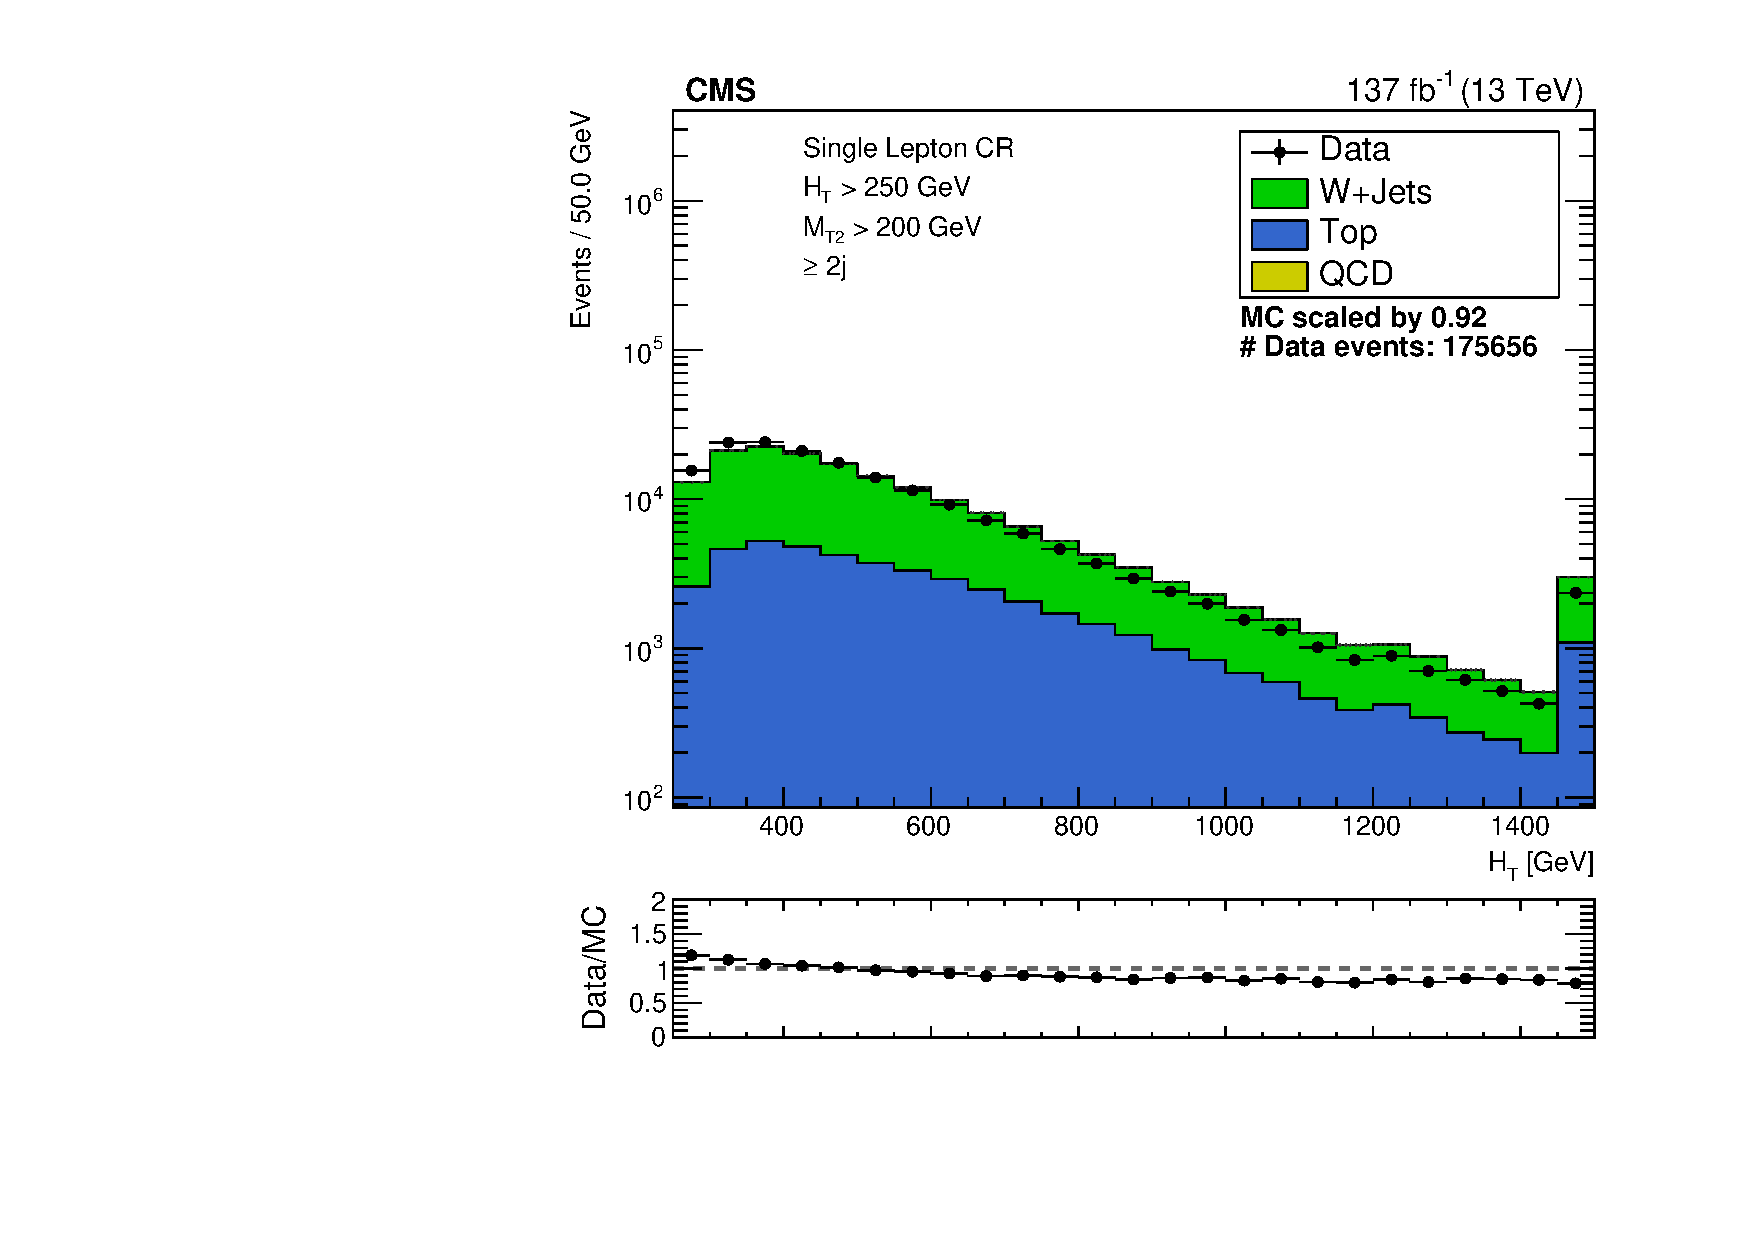
\includegraphics[width=0.47\textwidth]{figs/llep/crslbase_ht.pdf}
    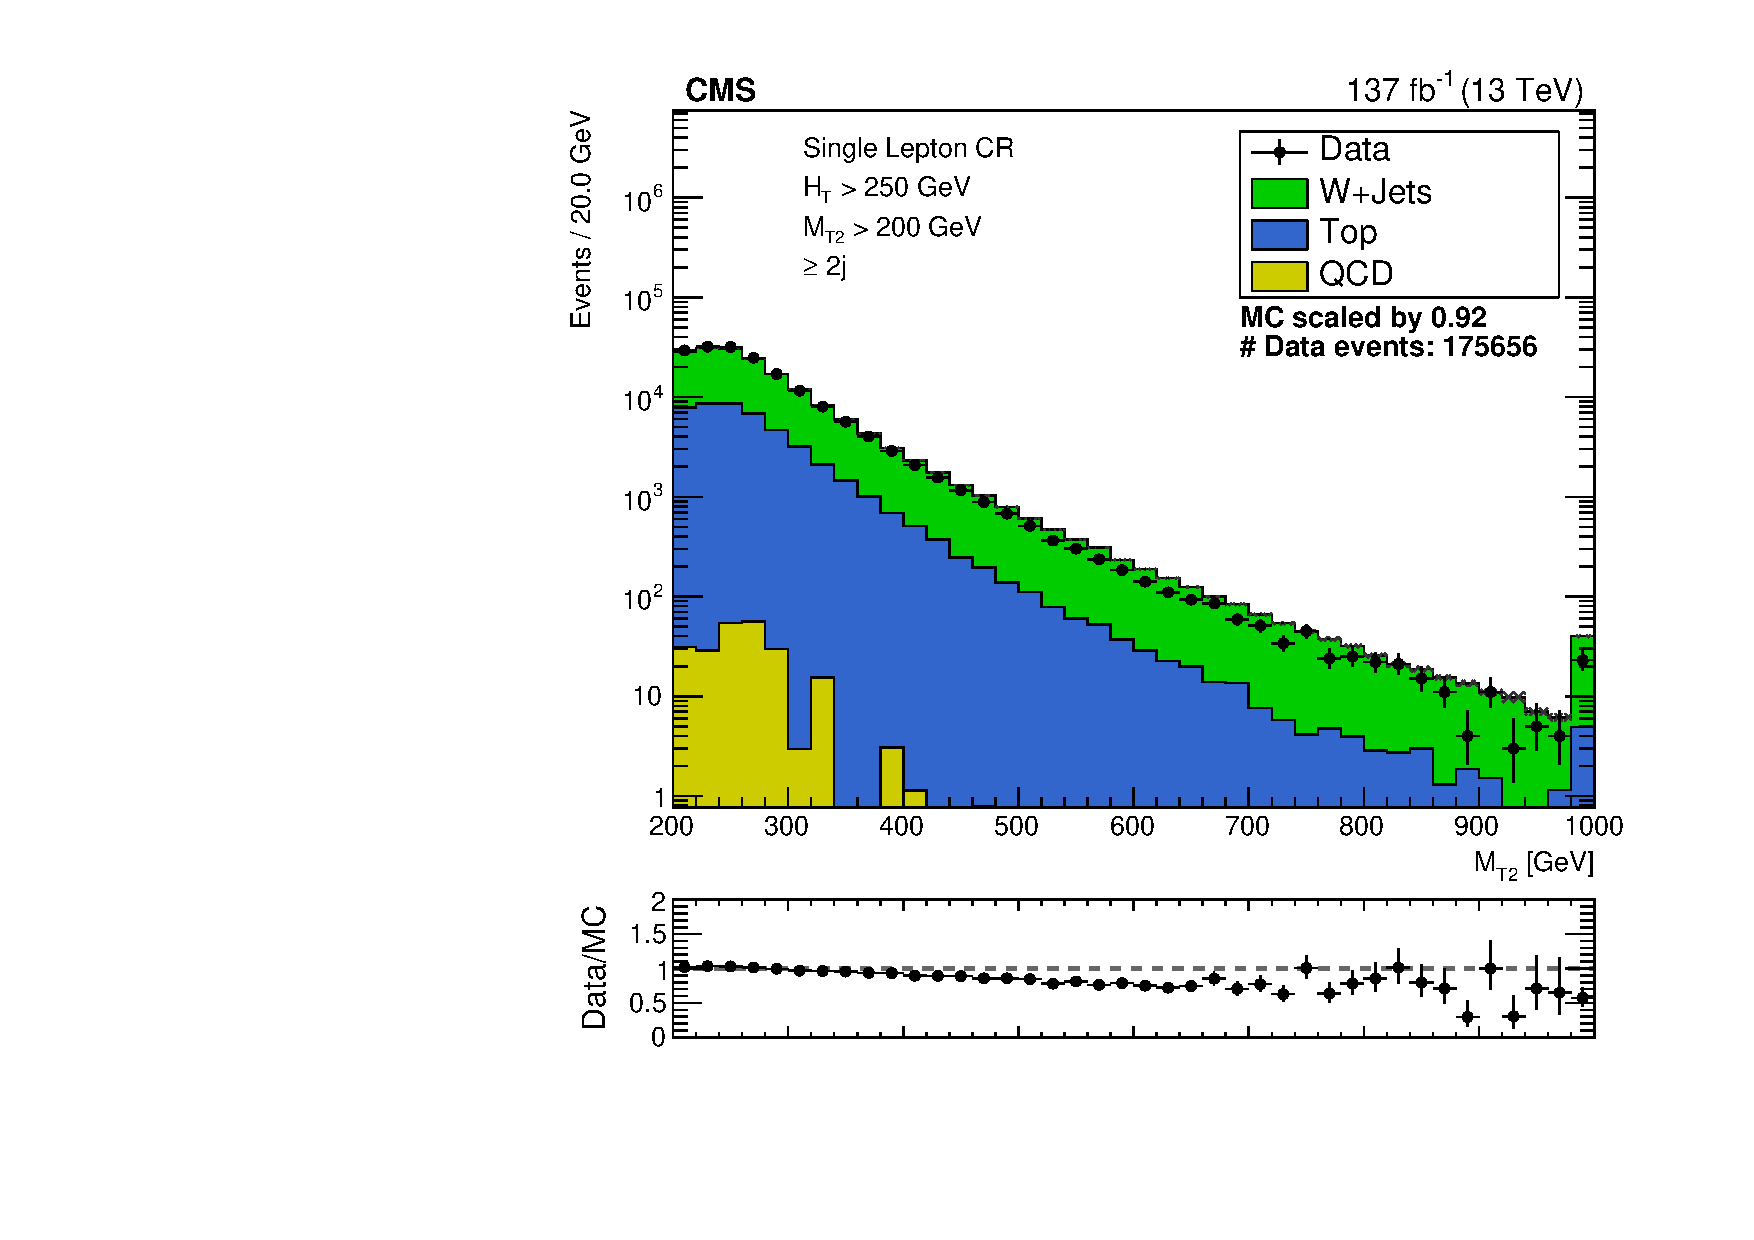
\includegraphics[width=0.47\textwidth]{figs/llep/crslbase_mt2.pdf} \\
    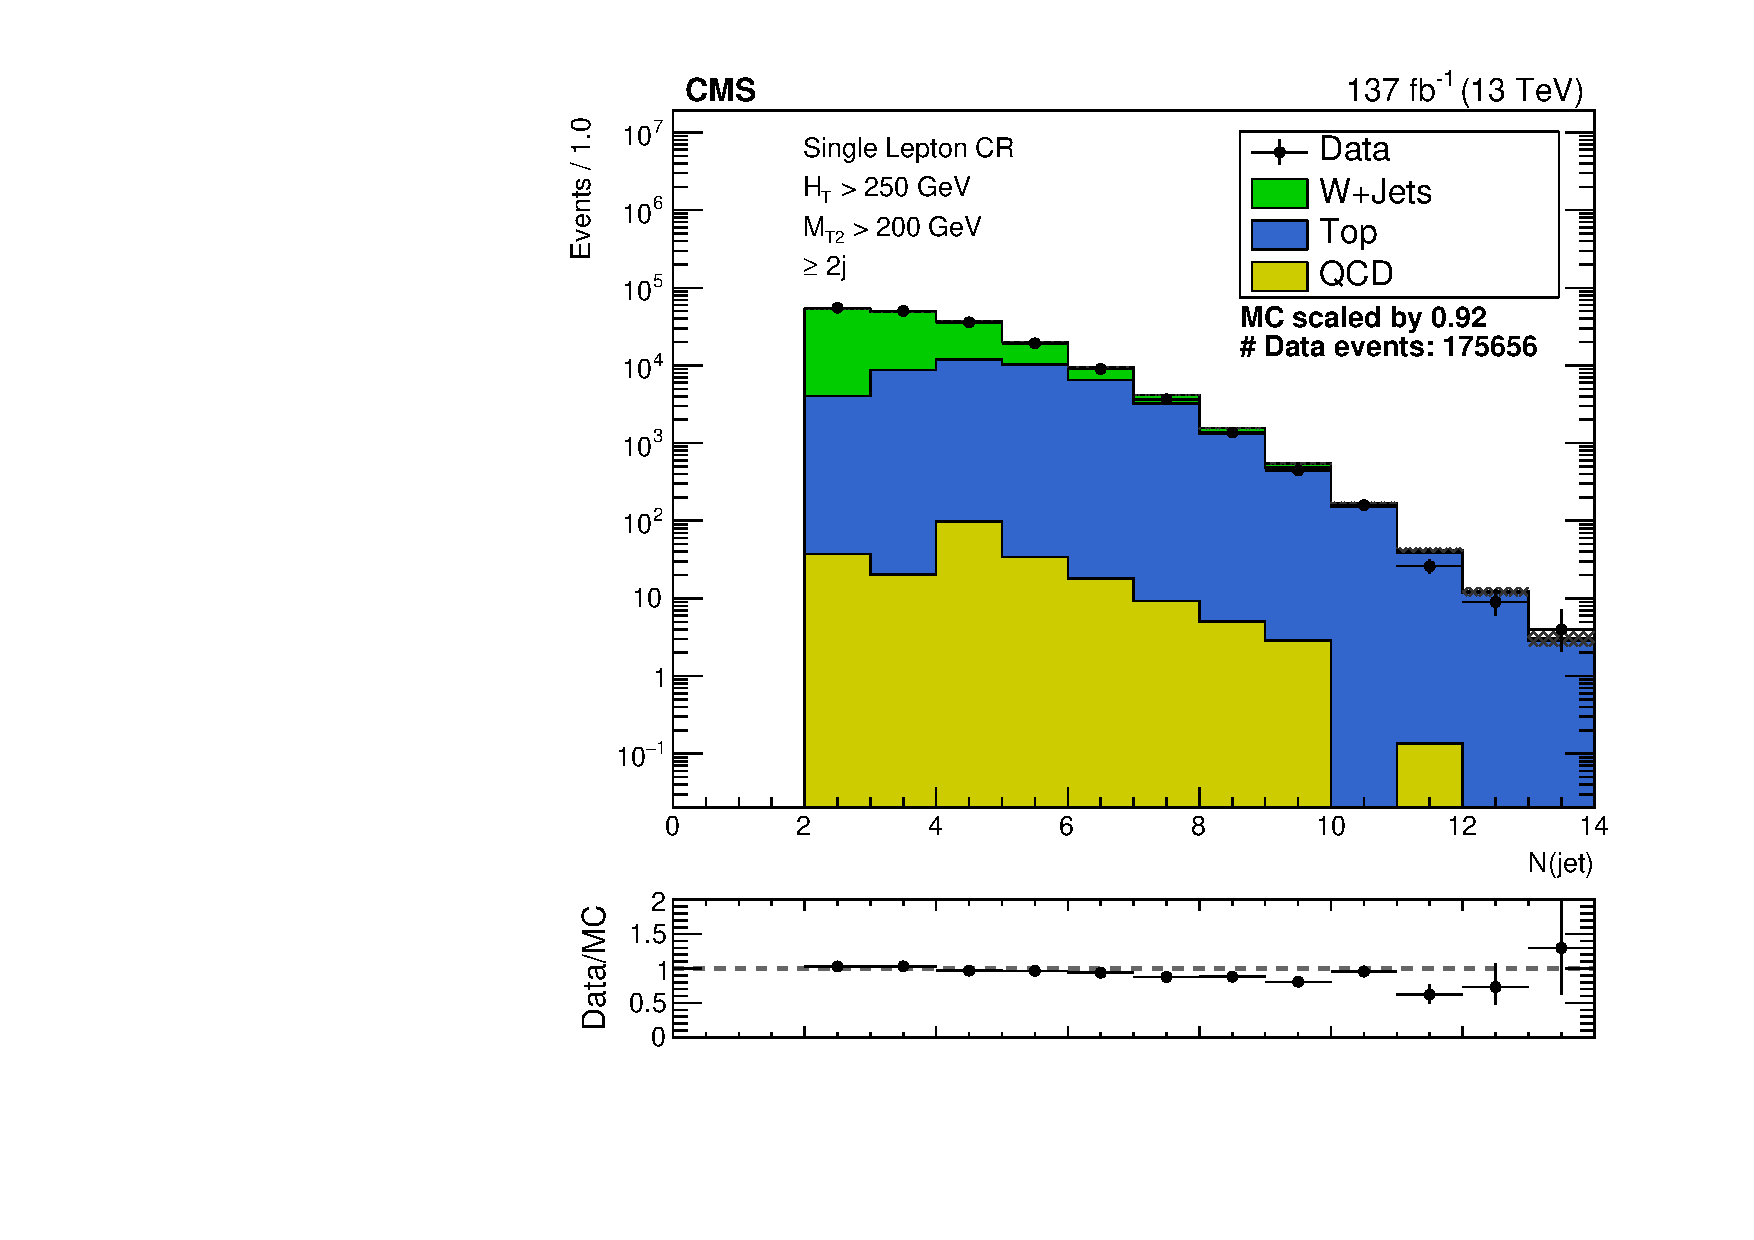
\includegraphics[width=0.47\textwidth]{figs/llep/crslbase_nJet30.pdf}
    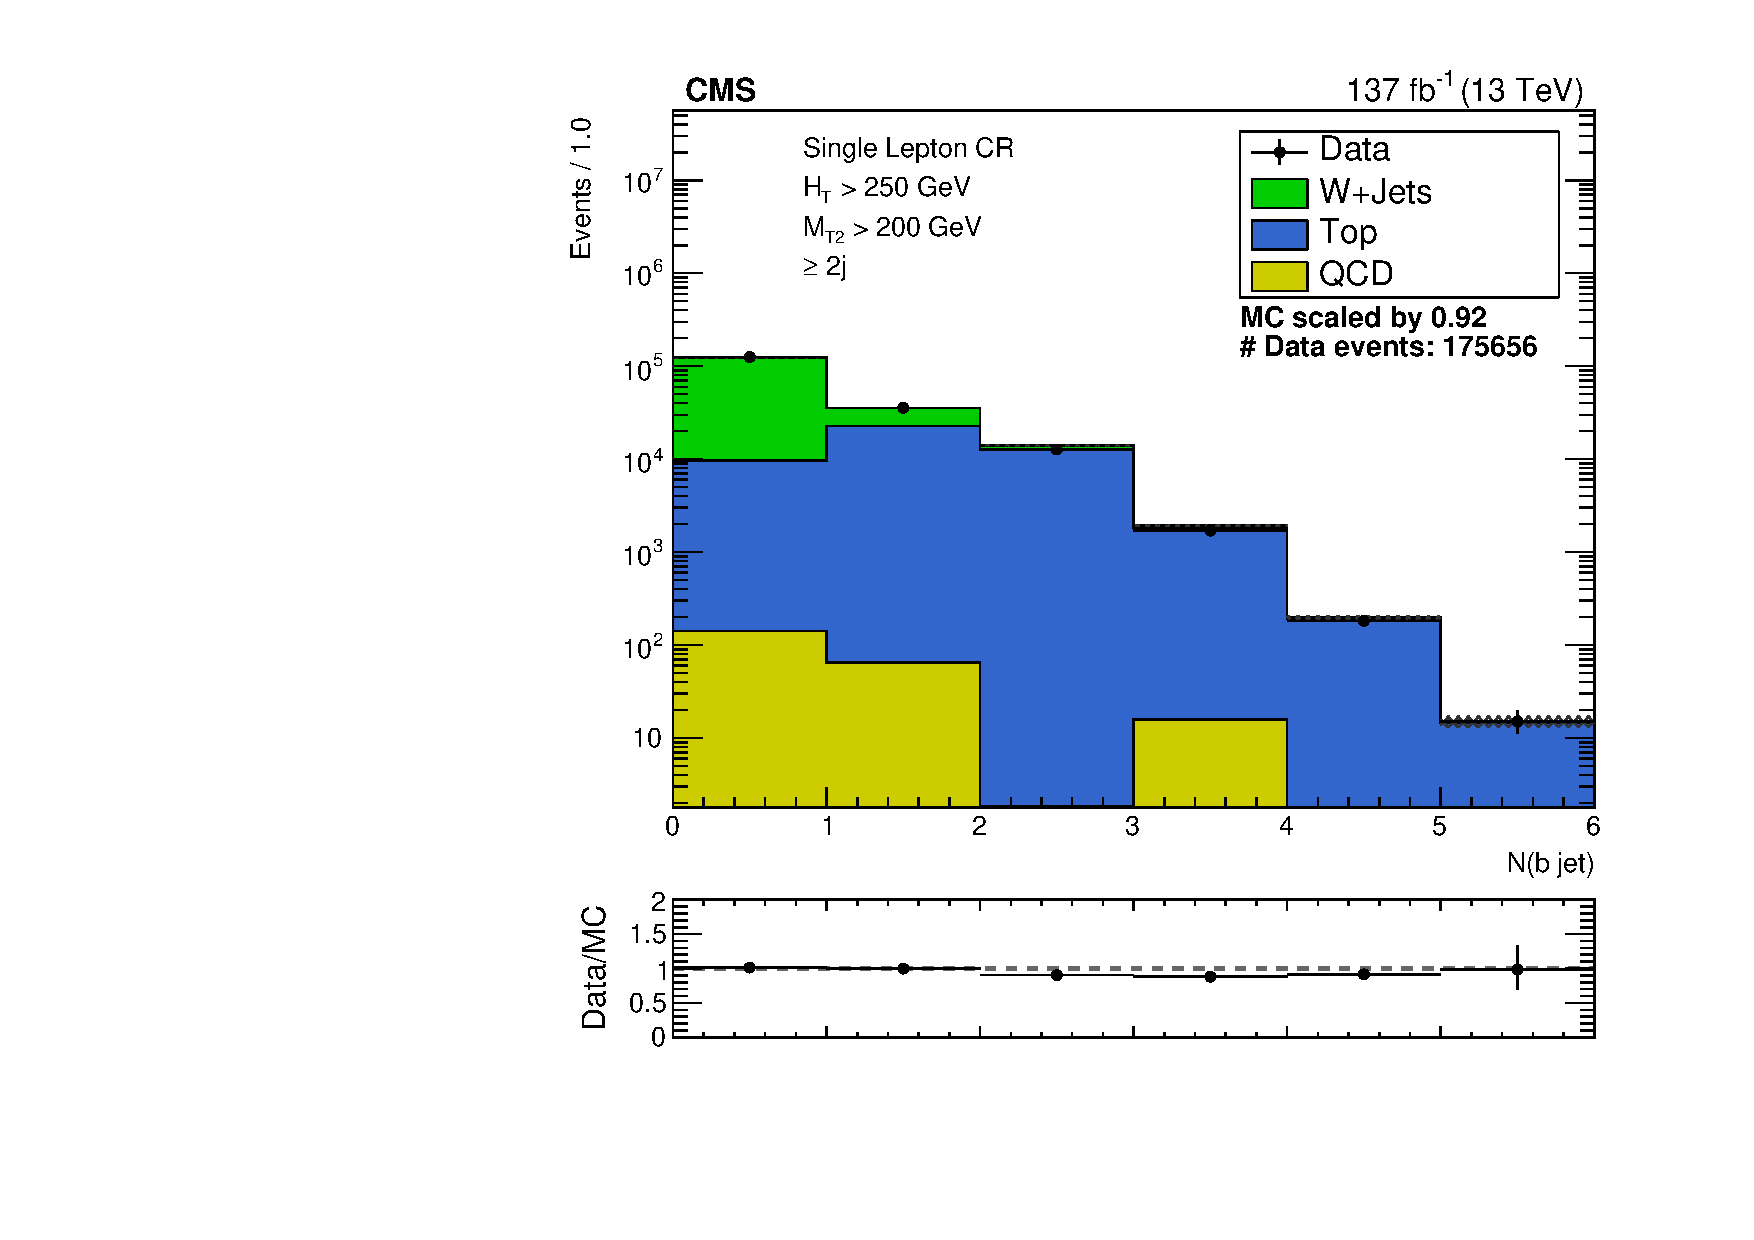
\includegraphics[width=0.47\textwidth]{figs/llep/crslbase_nBJet20.pdf} \\
    \caption{Data vs.\ MC comparisons in the baseline single lepton control region, for $\Nj\geq2$.
      From left to right, top to bottom, the variables
      plotted are \Ht, \mttwo, \Nj, and \Nb.
            }
    \label{fig:llep_crplots}
  \end{center}
\end{figure}

As with the \znunu estimate,
the lost lepton estimate is first performed in each $(\Ht,\Nj,\Nb)$ topological region, integrated
over \mttwo (for the monojet region, the \Ht dimension is equivalent to $\vSS{p}{T}{\mrm{jet1}}$,
so there is no integration and the estimate is performed in each analysis bin). For all regions
with 7--9 or $\geq$10 jets and $\geq$1 b tag, an inclusive control region with $\geq$7 jets and 1--2 b tags
is used, to avoid low statistics and higher signal contamination in regions with high jet and b-jet multiplicity.
Similarly, regions with either 7--9 or $\geq$10 jets and 0 b tags are all predicted using control region bins
with $\geq$7 jets and 0 b tags, due to low control regions statistics in regions with $\geq$10 jets.

Fig.~\ref{fig:llep_njextrap} shows \Nj distributions for data and MC in the $\geq$7 jet region, for both $\Nb=0$
and $\Nb\geq1$. Good agreement is observed, justifying the use of MC to extrapolate into the $\geq$10 jet regions
as described above. For the $\Nb$ distributions, agreement is not as good, so a reweighting is performed to correct
MC as described in the following section.

\begin{figure}[ht]
  \begin{center}
    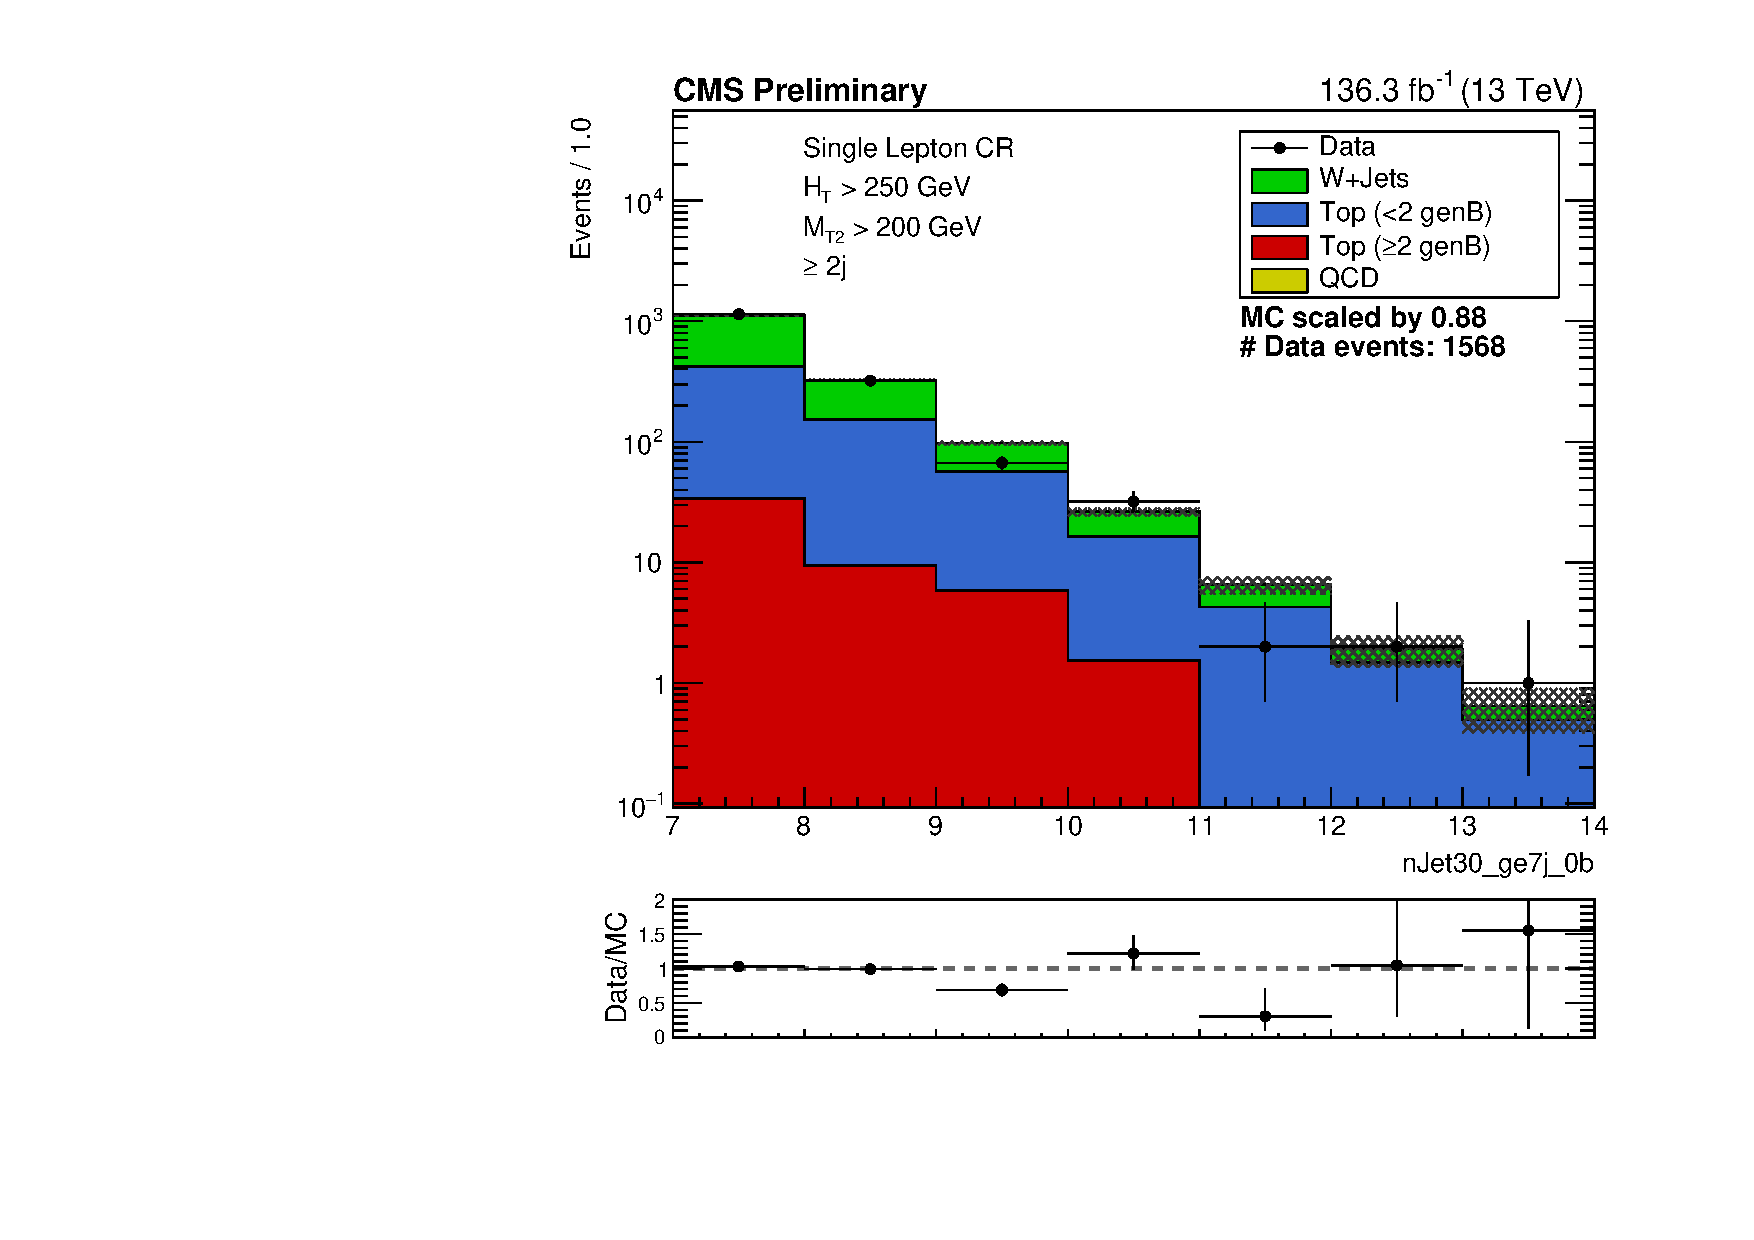
\includegraphics[width=0.47\textwidth]{figs/llep/crslbase_nJet30_ge7j_0b.pdf}
    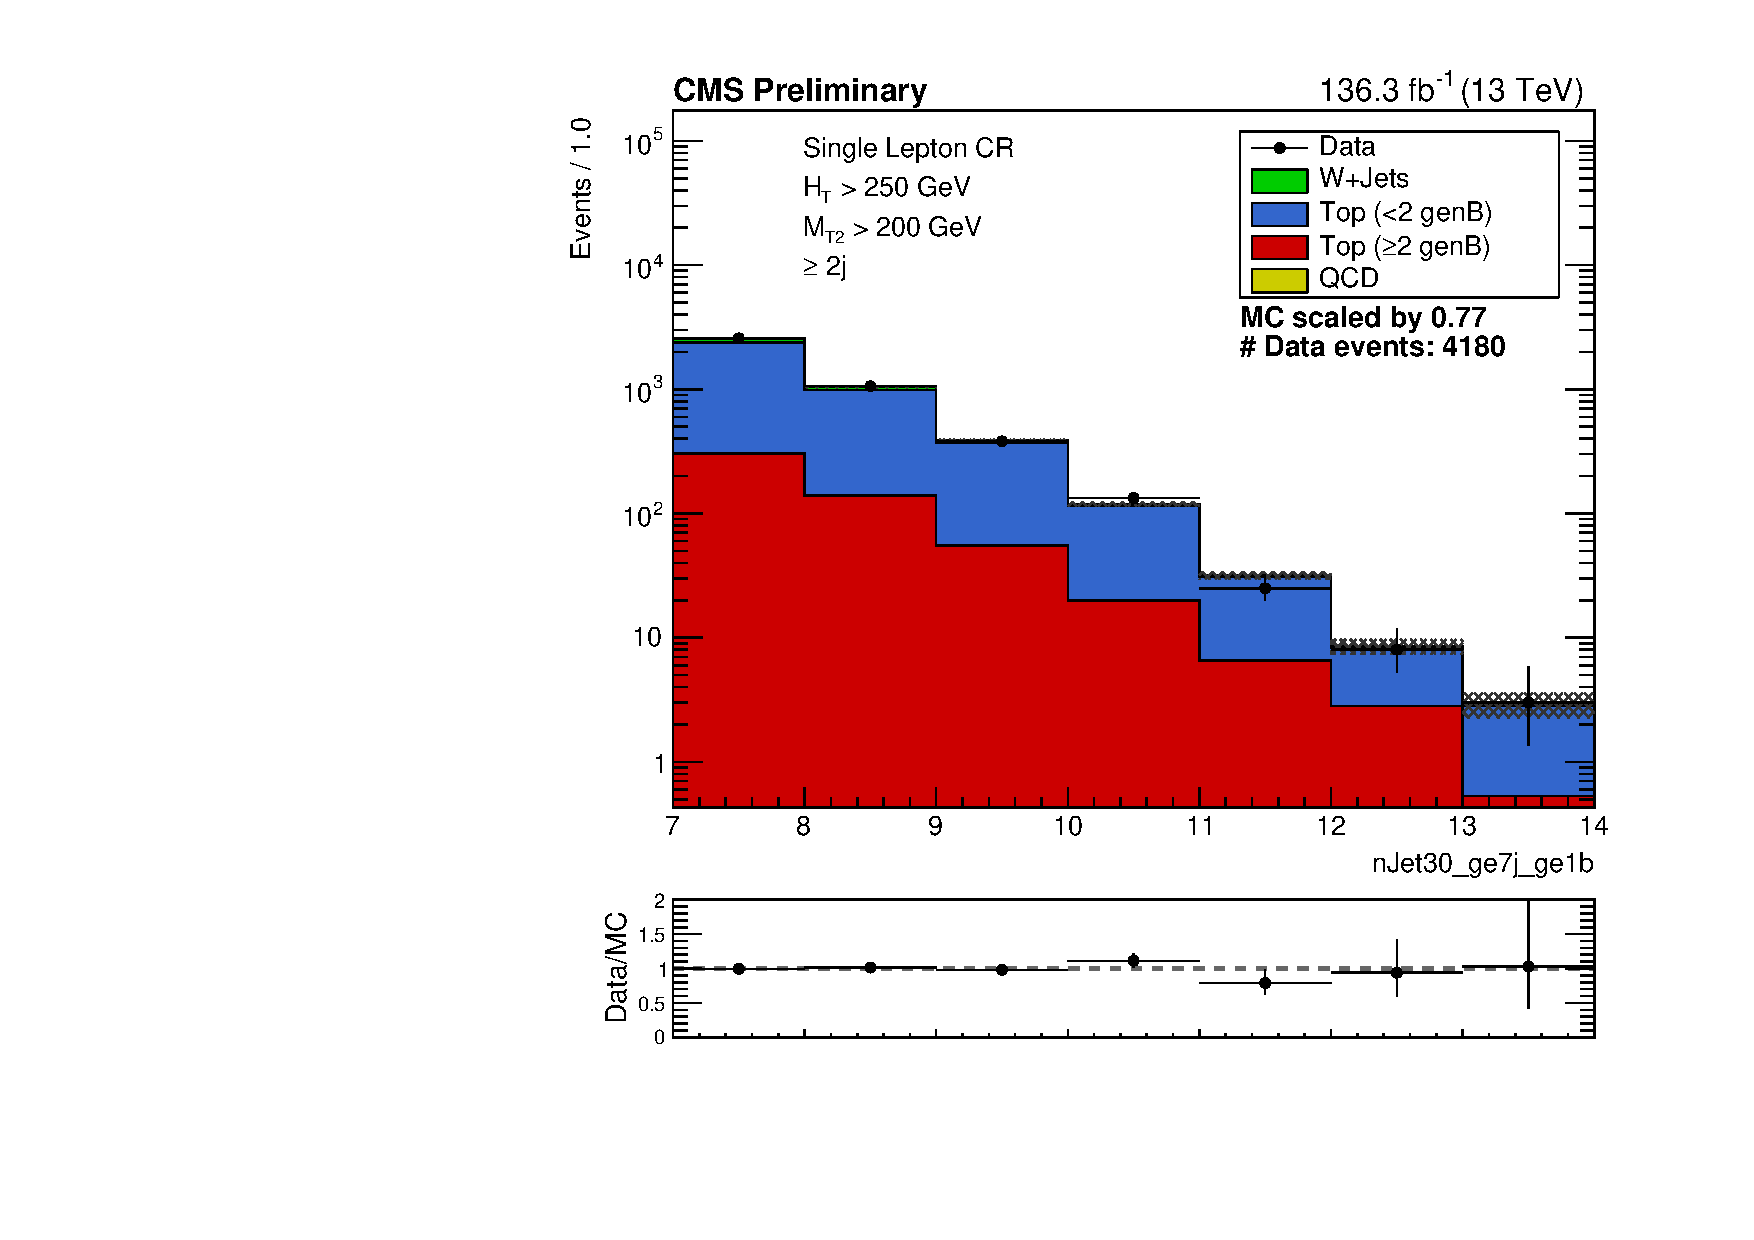
\includegraphics[width=0.47\textwidth]{figs/llep/crslbase_nJet30_ge7j_ge1b.pdf}
    \caption{Data vs.\ MC \Nj comparisons in the baseline single lepton control region with $\Nj\geq7$,
      for $\Nb=0$ (left) and $\Nb\geq1$ (right). Agreement is sufficient to justify using MC to extrapolate
      along the \Nj dimension for high-\Nj regions.
            }
    \label{fig:llep_njextrap}
  \end{center}
\end{figure}

For regions with $\Ht>1500\GeV$, all events with
$\mttwo>200\GeV$ are used in the control region even though the signal region starts at $\mttwo>400\GeV$.
Once the per-topological region estimate is done, a hybrid approach using both data and MC is
used to extrapolate along the \mttwo dimension, as described in Sec.~\ref{sec:zinv_mt2}.

The final estimate in each $(\Ht,\Nj,\Nb,\mttwo)$ signal region can then be summarized as
\be\label{eq:llep_est}
N_{\mrm{LL}}^\mrm{SR} = N_\mrm{1\ell}^\mrm{CR}(\mttwo,\Omega)\; R_\mrm{MC}^{0\ell/1\ell}(\mttwo,\Omega)\;
k_\mrm{LL}(\mttwo|\Omega),
\ee
where
\begin{itemize}\setlength\itemsep{0mm}
\item $N_\mrm{1\ell}^\mrm{CR}$ is the number of observed events in data in the single lepton control region.
\item $R_\mrm{MC}^{0\ell/1\ell}$ is the ratio between zero lepton and single lepton MC yields in this region.
\item $k_\mrm{LL}(\mttwo|\Omega)$ is a normalized template used to distribute events as a function
of \mttwo in each topological region (see Sec.~\ref{sec:llep_mt2}), only necessary in regions with $\geq$2 jets.
\end{itemize}



\subsection{$\ttbar+\text{heavy flavor}$ modeling}
\label{sec:llep_ttbb}
As described previously, regions with $\geq$7 jets and $\geq$1 b tag, are predicted
using a single control region with $\geq$7 jets and 1--2 b tags. MC is then used to
extrapolate both into the $\geq$10 jet region and into the high-\Nb regions.
While the MC modeling of \Nj is sufficient out-of-the-box (Fig.~\ref{fig:llep_njextrap}),
this is not the case for \Nb modeling. Fig.~\ref{fig:llep_nbextrap} (left) shows a comparison
of \Nb in data and MC in the $\geq$7 jet portion of the single lepton control region.
At high \Nb, MC under-predicts the number of events in data by a significant amount.

This disagreement can be attributed to known MC mis-modeling of $\ttbar+\text{heavy flavor}$
events (i.e. $\ttbar b\bar{b}+X$). A CMS measurement of the ratio 
$\sigma(\ttbar b\bar{b})/\sigma(\ttbar jj)$ finds that this ratio is a factor of $1.7\pm0.5$ higher
in data than in MC~\cite{TOP_ttbb}. Hence, to correct for this we identify \ttbar and $\ttbar\mrm{V}$ MC
events with two additional generator-level b jets not from top decay, and weight them by an additional
factor of $1.7\pm0.5$. The uncertainty is propagated to the final estimate as a systematic uncertainty.
Fig.~\ref{fig:llep_nbextrap} (right) shows the \Nb distribution after this reweighting procedure, and
one sees that agreement is significantly improved.

\begin{figure}[ht]
  \begin{center}
    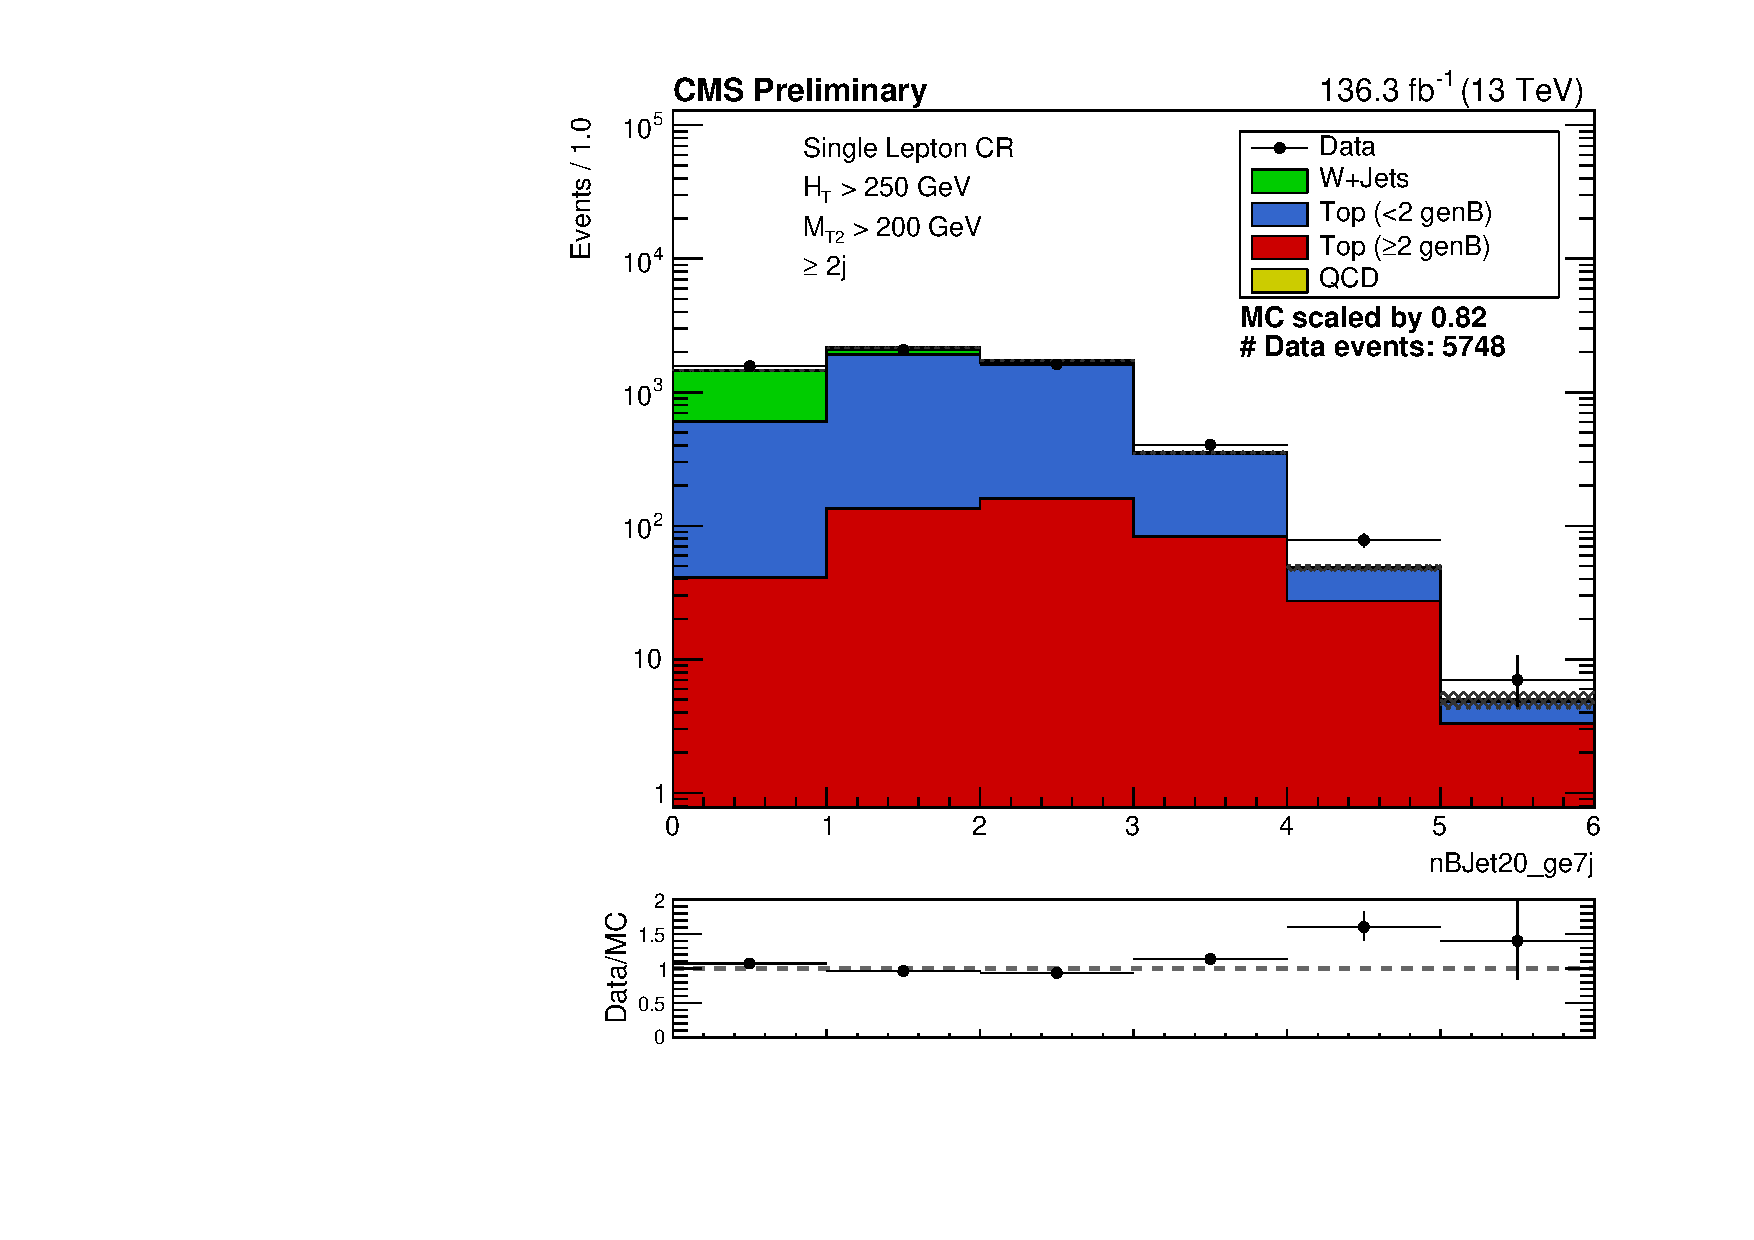
\includegraphics[width=0.47\textwidth]{figs/llep/crslbase_nBJet20_ge7j_ttbbNonWeighted.pdf}
    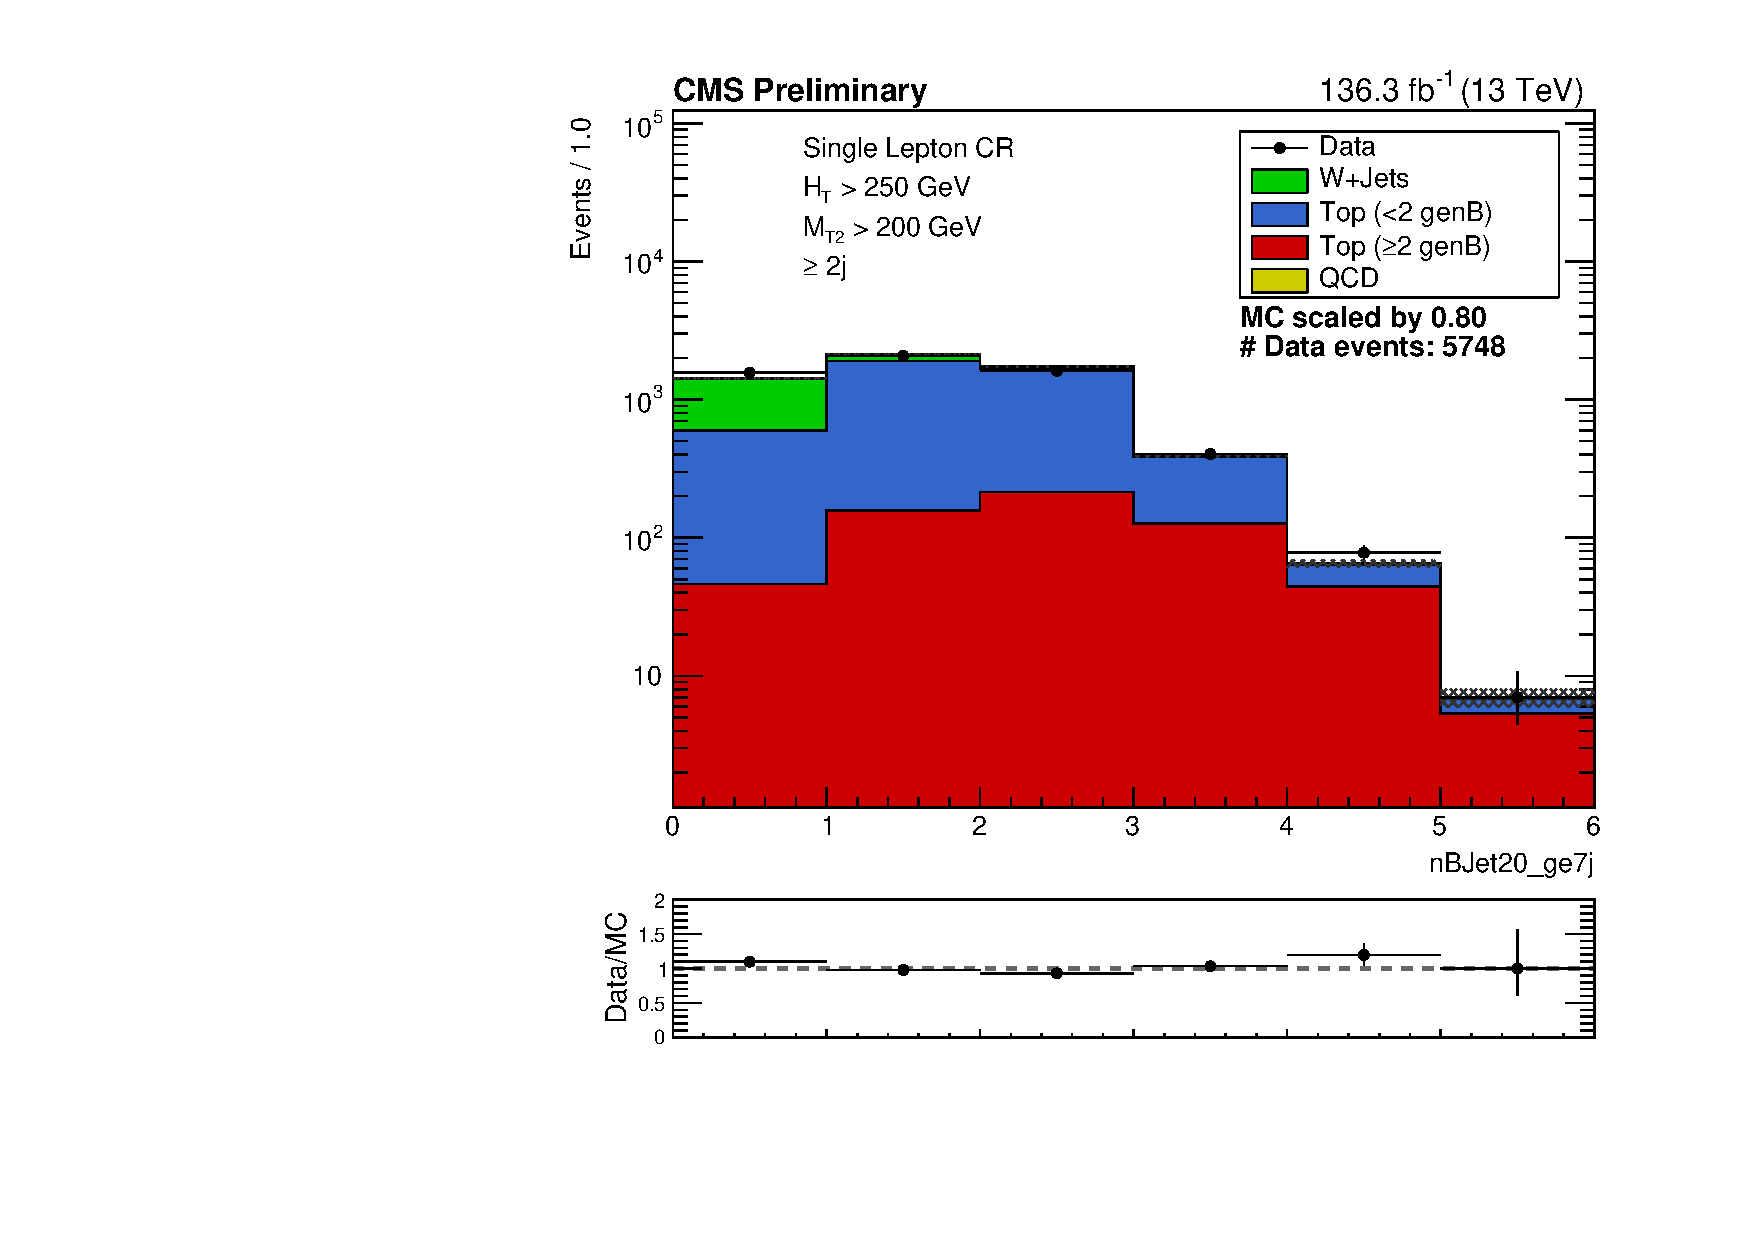
\includegraphics[width=0.47\textwidth]{figs/llep/crslbase_nBJet20_ge7j_ttbbWeighted.pdf}
    \caption{Data vs.\ MC \Nb comparisons in the baseline single lepton control region with $\Nj\geq7$,
      with no extra weights (left) and with the $\ttbar b\bar{b}$ component (red) scaled by 1.7 (right), as described
      in Sec.~\ref{sec:llep_ttbb}. The reweighting significantly improves agreement in the high-\Nb bins.
            }
    \label{fig:llep_nbextrap}
  \end{center}
\end{figure}

\subsection{Signal contamination}
Despite the selections intended to reduce contributions from signal to the single lepton control
regions, signal contamination can be non-negligible in some regions of phase space where the
signal is kinematically similar to the background. A contribution from signal to the control
region would result in an overestimation of the lost lepton background.

The only signals considered in this analysis which show potential contamination issues are those with prompt lepton decays. 
Namely, gluino pair production where the gluinos decay to top quarks, and direct top squark pair production where the squarks decay to top quarks. 
The contributions from other signals are found to be negligible in the control
regions. For points near the expected exclusion limits at high masses, the signal contamination
is maximally 5\% of the expected background yields in the control regions, including the hybrid \mttwo binning described in the following section. 
The main place where this effect becomes significant is for top squark pair production points
in which the mass difference between the top squark and neutralino is near the top quark mass, such that the
signal looks very similar to SM \ttbar production.

To account for this in our interpretations, we treat the amount by which the lost lepton background 
would be overestimated as a reduction in signal efficiency. Specifically, in each analysis bin, we define
\be
N_\mrm{sig}^\mrm{SR'} = N_\mrm{sig}^\mrm{SR} - TF\cdot N_\mrm{sig}^\mrm{CR},
\ee
where $N_\mrm{sig}^\mrm{SR}$ and $N_\mrm{sig}^\mrm{CR}$ are the predicted signal in the signal region and control region bins,
respectively, and $TF$ is the transfer factor from control to signal region used in the lost lepton estimate (in
the notation of Eq.~\ref{eq:llep_est}, $TF=R_\mrm{MC}^{0\ell/1\ell}\cdot k_\mrm{LL}(\mttwo|\Omega)$).
Then the quantity $N_\mrm{sig}^\mrm{SR'}\leq N_\mrm{sig}^\mrm{SR}$ is used in calculating the limit on the
signal cross section.

This treatment has been used in several other CMS SUSY analyses (e.g.~\cite{SUS_stop1l}),
and has the useful property that $N_\mrm{sig}^\mrm{SR'}$ depends linearly on the signal cross section. 
This can be seen by rewriting as
\be
N_\mrm{sig}^\mrm{SR'} = \sigma_\mrm{sig}\cdot\mathcal{L}\cdot
(\varepsilon_\mrm{sig}^\mrm{SR} - TF\cdot\varepsilon_\mrm{sig}^\mrm{CR}),
\ee
where $\sigma_\mrm{sig}$ is the signal cross section, $\mathcal{L}$ is the integrated luminosity, and
$\varepsilon_\mrm{sig}^\mrm{SR}$ and $\varepsilon_\mrm{sig}^\mrm{CR}$ are the efficiencies for the signal to
populate the signal and control regions, respectively.

\section{\texorpdfstring{\mttwo}{MT2} extrapolation}
\label{sec:llep_mt2}

In a similar way as the \znunu background estimate, the control region prediction in each topological region is
extrapolated along the \mttwo dimension using a data/MC ``hybrid'' shape template.
Starting from the highest \mttwo bin in each (\Ht,\Nj,\Nb) control region, we merge with lower bins until
there are at least 50 expected MC events in the merged bin. 

Lower \mttwo bins with large statistics are used directly
to predict the backgrounds, so $N_\mrm{1\ell}^\mrm{CR}$ and $R_\mrm{MC}^{0\ell/1\ell}$ are measured in the specific
\mttwo bin and $k_\mrm{LL}(\mttwo|\Omega)$ is equal to 1.
For the higher \mttwo bins past the merging threshold, the control region is integrated over the merged bin
for the purposes of computing $N_\mrm{1\ell}^\mrm{CR}$ and $R_\mrm{MC}^{0\ell/1\ell}$. Then $k_\mrm{LL}$ is the 
ratio of the MC signal region yield in an individual \mttwo bin to that in the integrated bin (i.e., the \mttwo
shape within the merged bin is taken directly from signal region MC).

The MC modeling of \mttwo is checked in data, in single lepton events with either $\Nb=0$ or $\Nb\geq1$, as
shown in the left and right panels of Fig.~\ref{fig:llep_mt2dist}. The predicted distributions in the comparison
are obtained by summing all the relevant topological regions, after normalizing MC event yields to data
and distributing among the \mttwo bins using the procedure described above. The gray band in the ratio plot represents the
systematic uncertainty assessed to the predicted \mttwo shape, as described in the following section.
Fig.~\ref{fig:llep_mt2dist_ht} shows the same, but separately for each \Ht region.

\begin{figure}[t]
  \begin{center}
    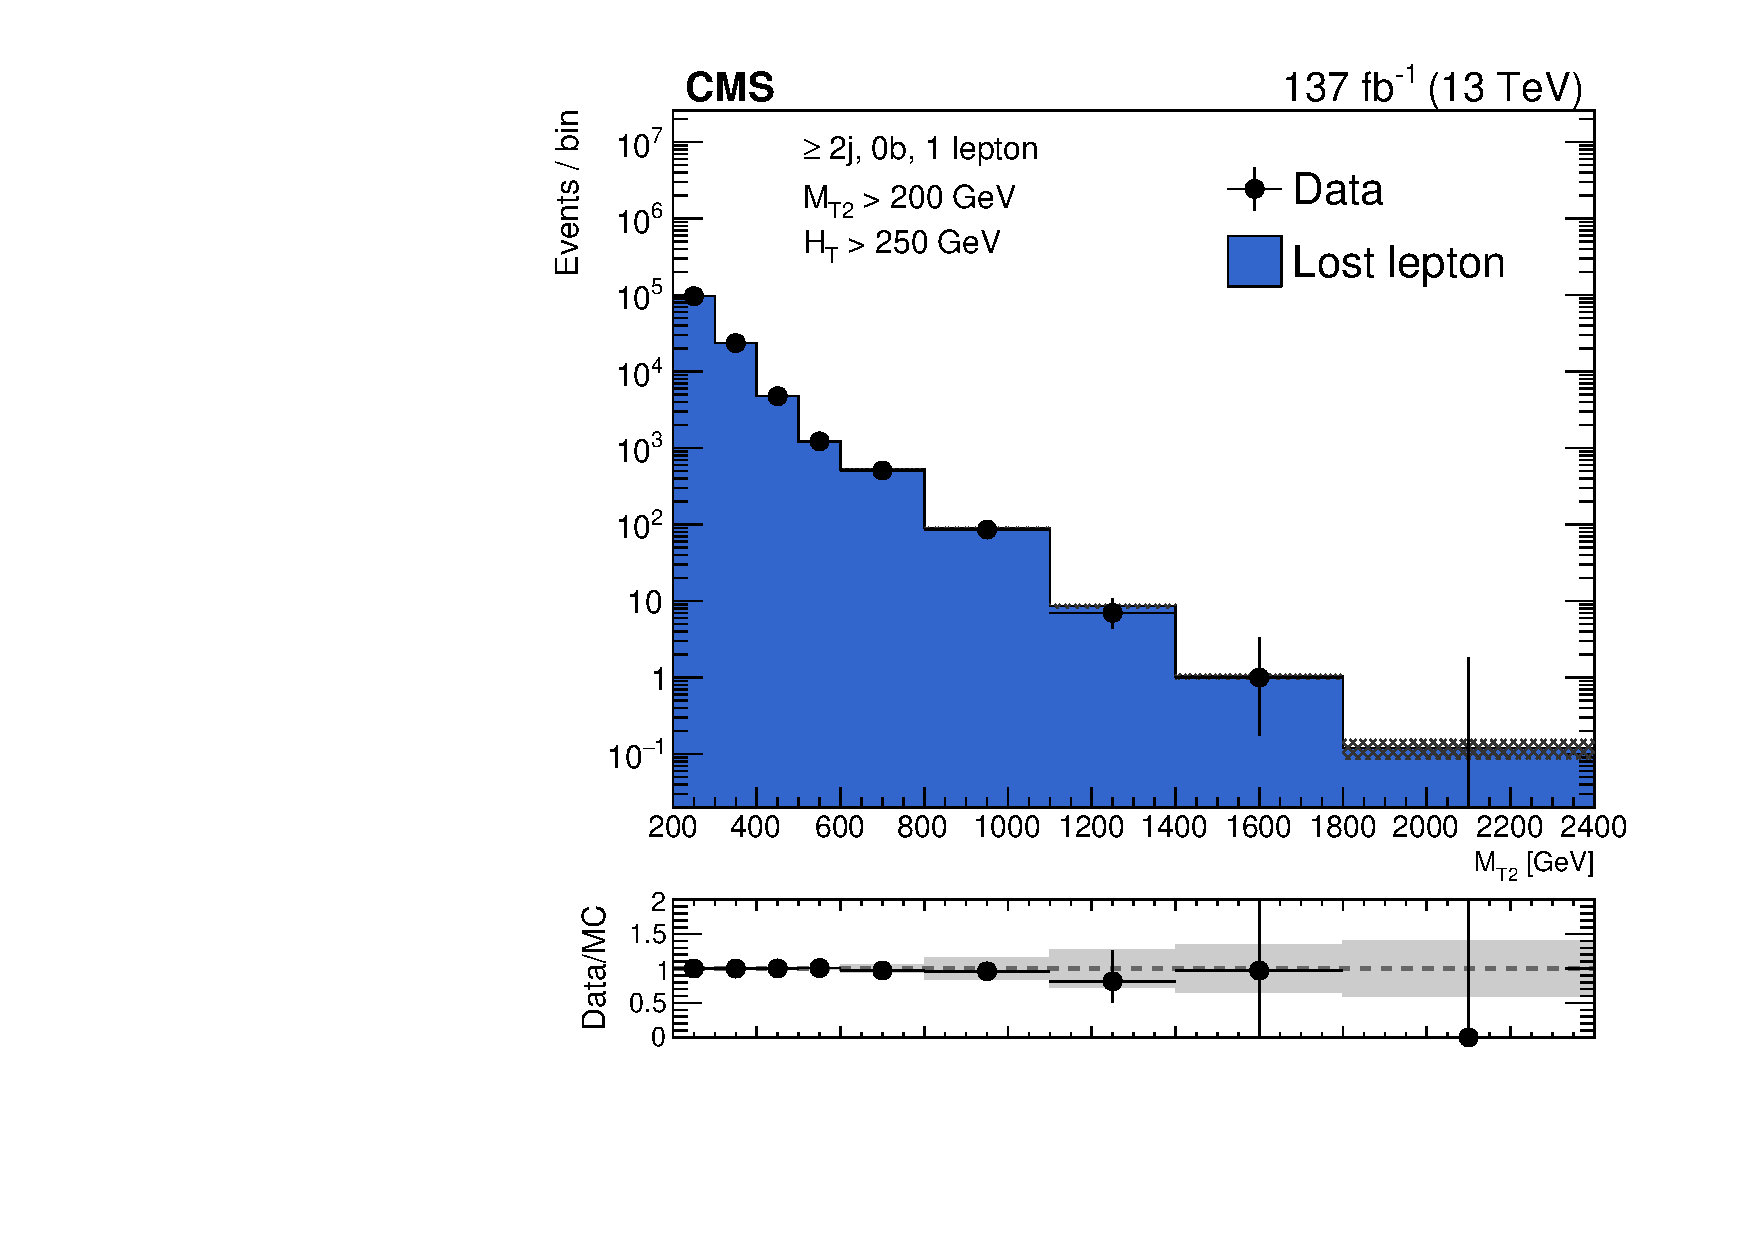
\includegraphics[width=0.47\textwidth]{figs/llep/lostlepHybrid_0b_mt2bins.pdf}
    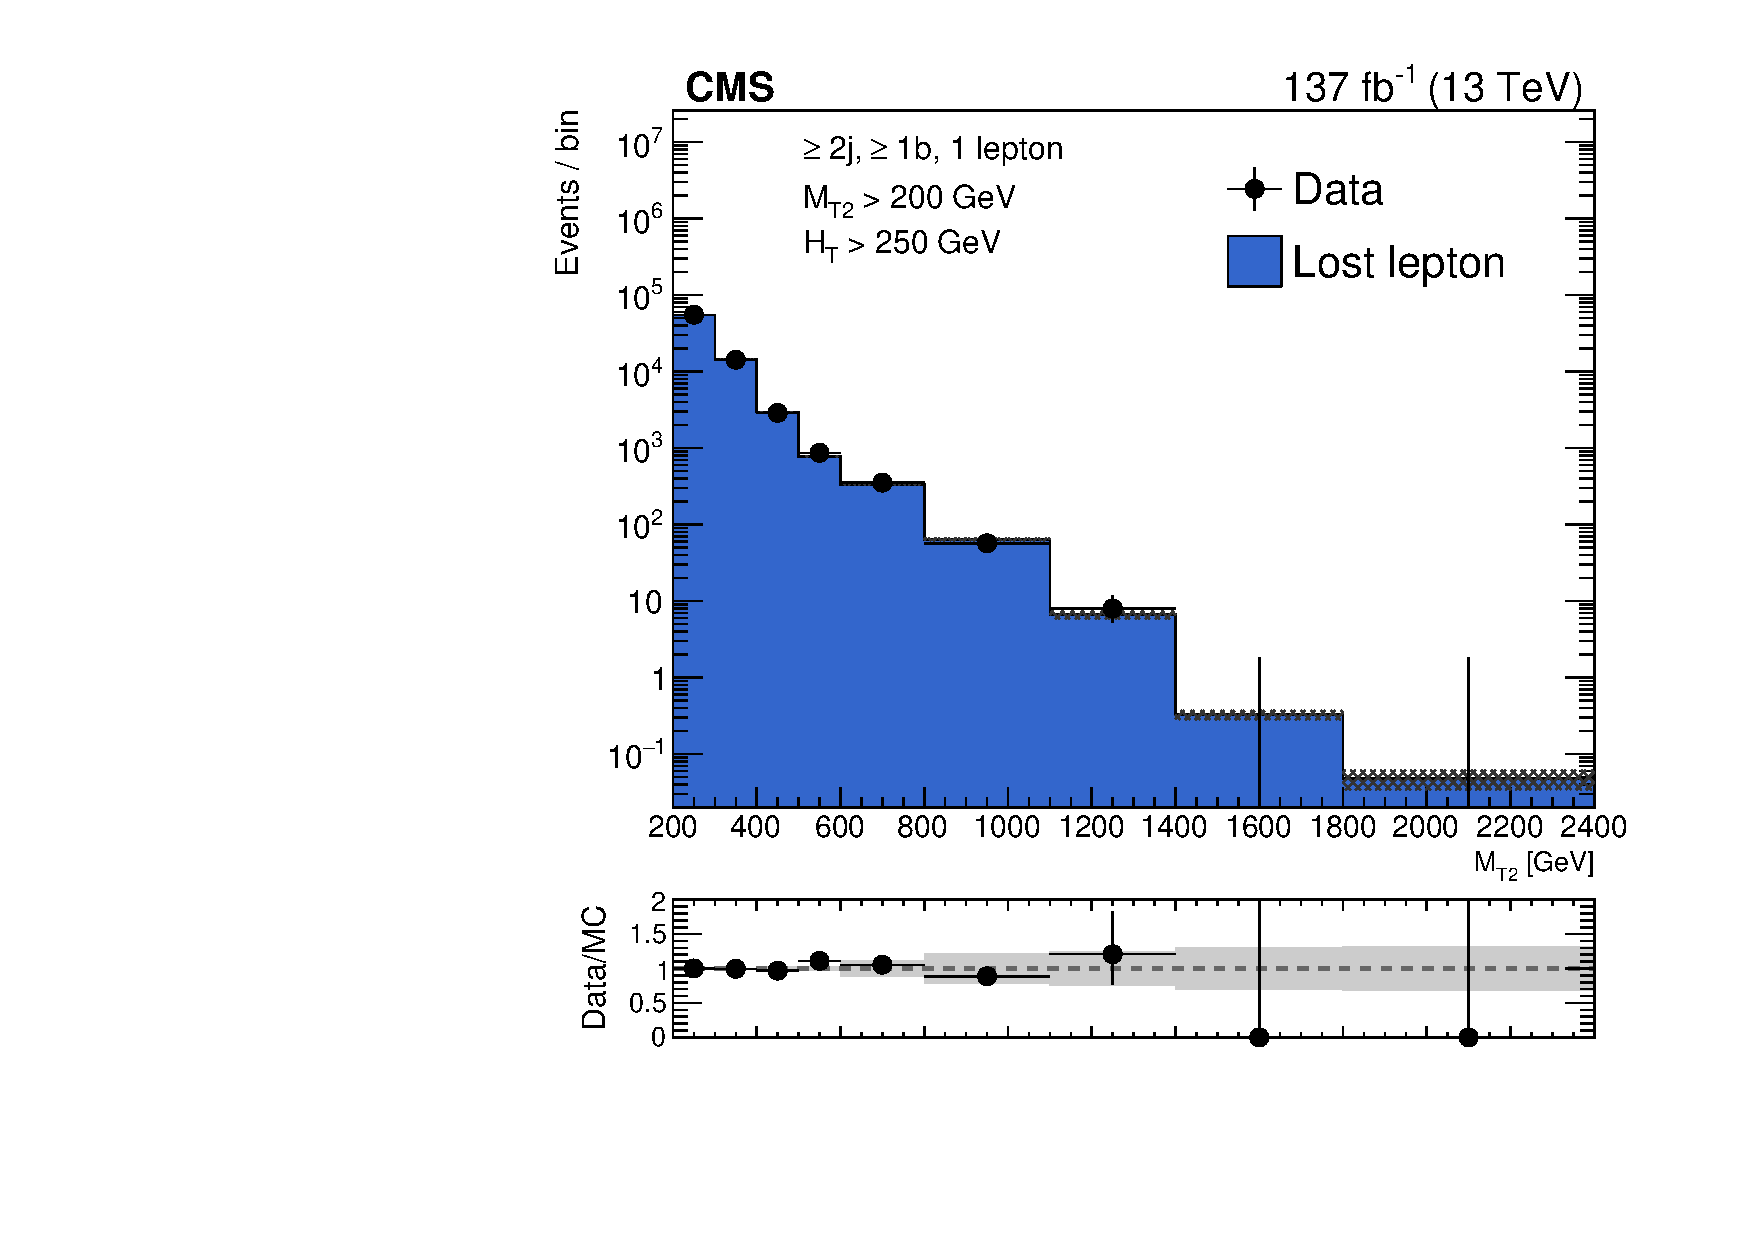
\includegraphics[width=0.47\textwidth]{figs/llep/lostlepHybrid_ge1b_mt2bins.pdf}
    \caption{Distributions of the \mttwo variable in data and MC for the single lepton control region,
      after normalizing the simulation to data in each topological region and distributing events
      among the \mttwo bins using the procedure described in Sec.~\ref{sec:llep_mt2}. On the left is a selection
      with $\Nb=0$, which probes mostly \wjets events, and on the right is a selection with $\Nb\geq1$, which
      probes primarily top quark processes. The solid gray band  in the ratio plot represents the
      systematic uncertainty assessed to the predicted \mttwo shape, as described in Sec.~\ref{sec:llep_syst}.
            }
    \label{fig:llep_mt2dist}
  \end{center}
\end{figure}

\begin{figure}[htbp]
  \begin{center}
    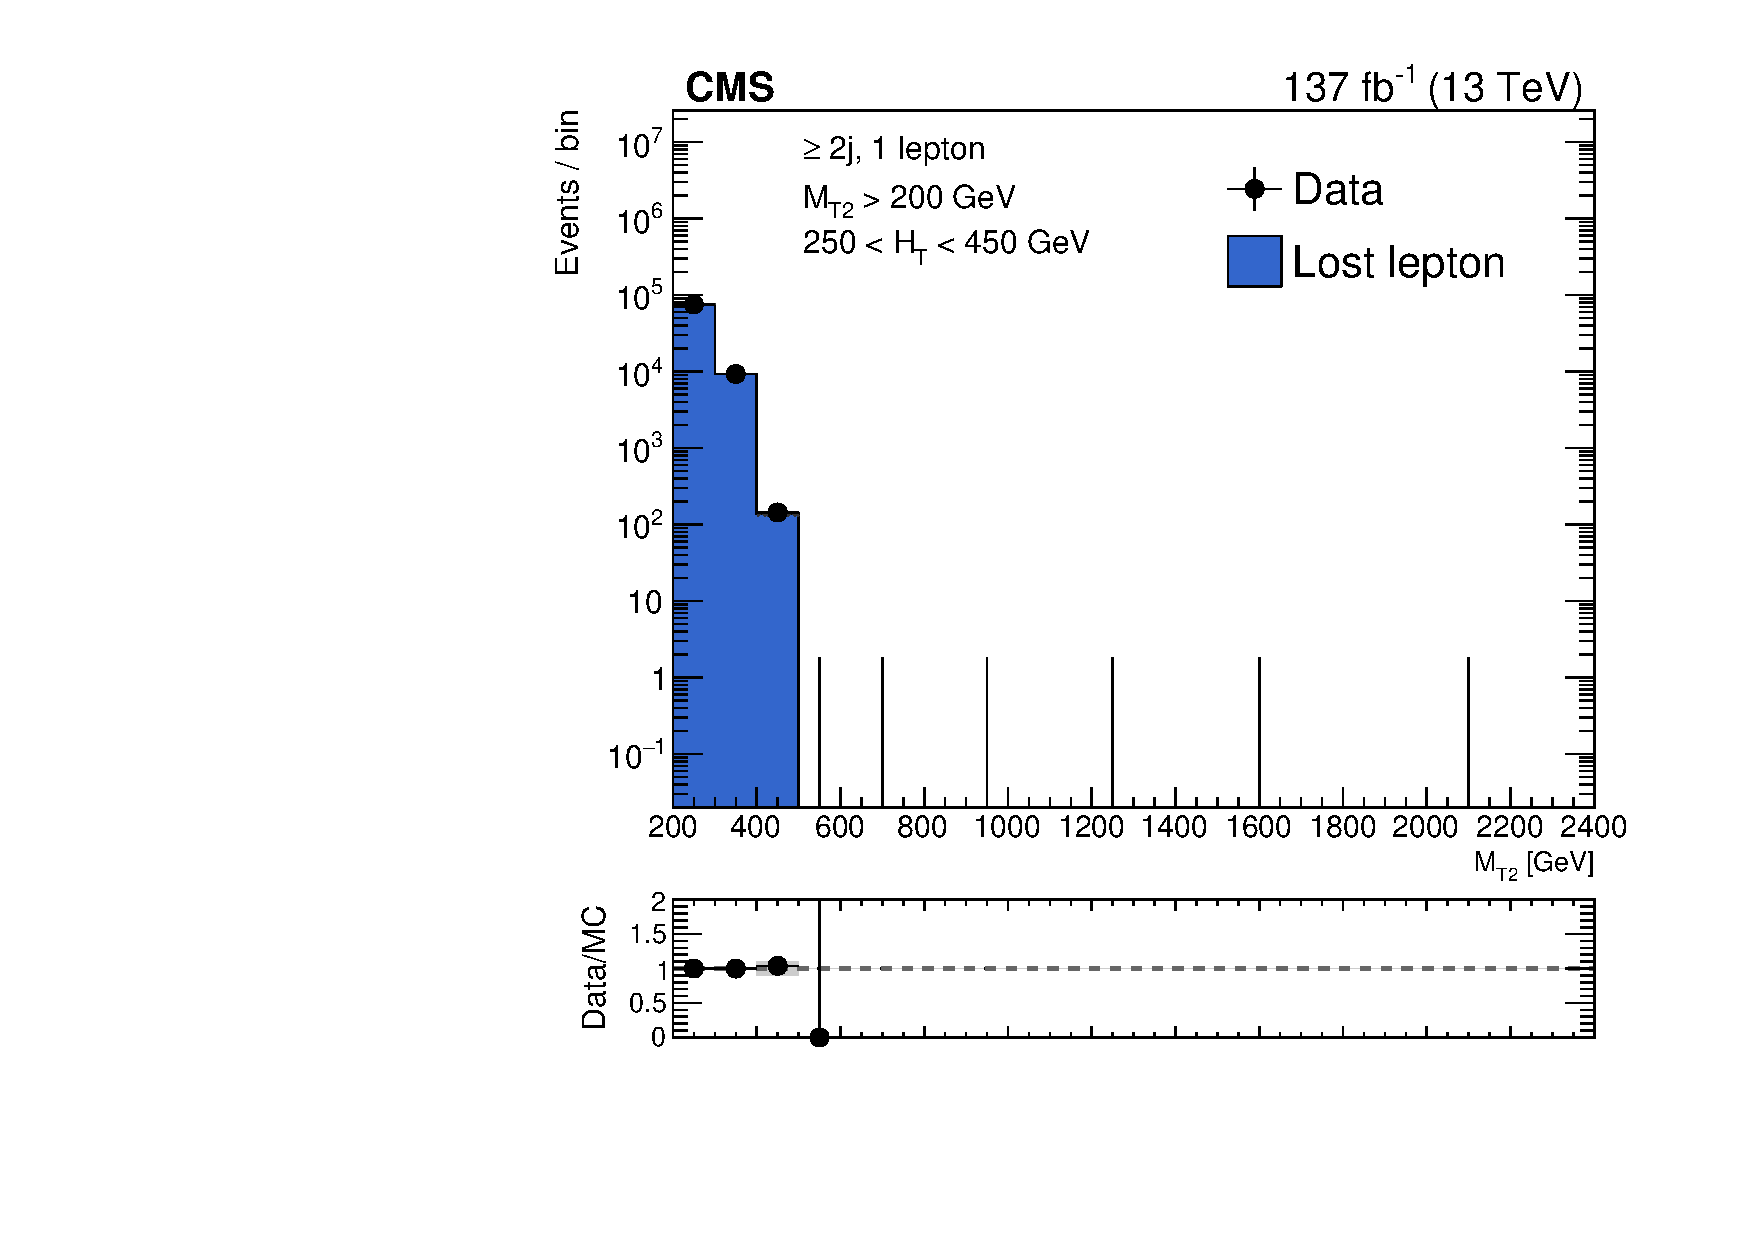
\includegraphics[width=0.47\textwidth]{figs/llep/lostlepHybrid_incl_HT250to450_mt2bins.pdf}
    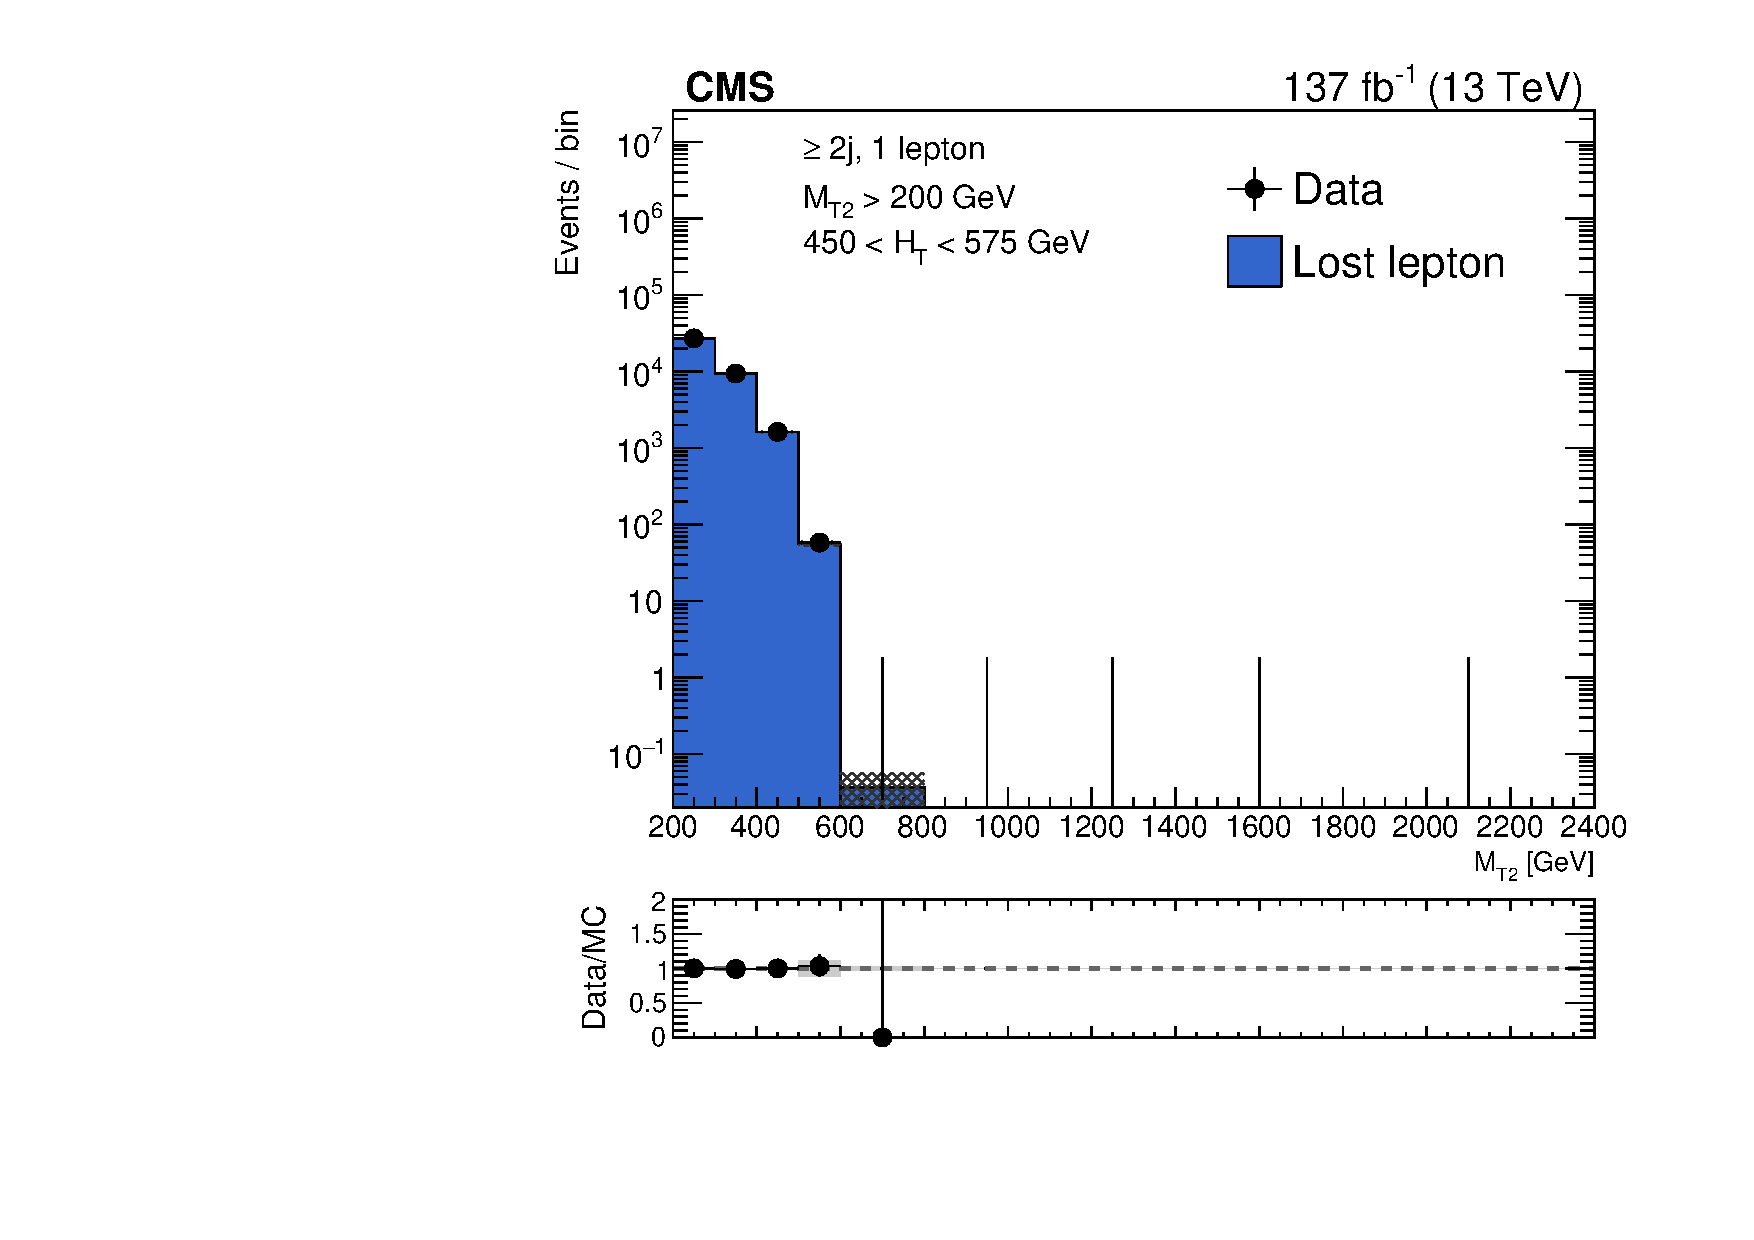
\includegraphics[width=0.47\textwidth]{figs/llep/lostlepHybrid_incl_HT450to575_mt2bins.pdf} \\
    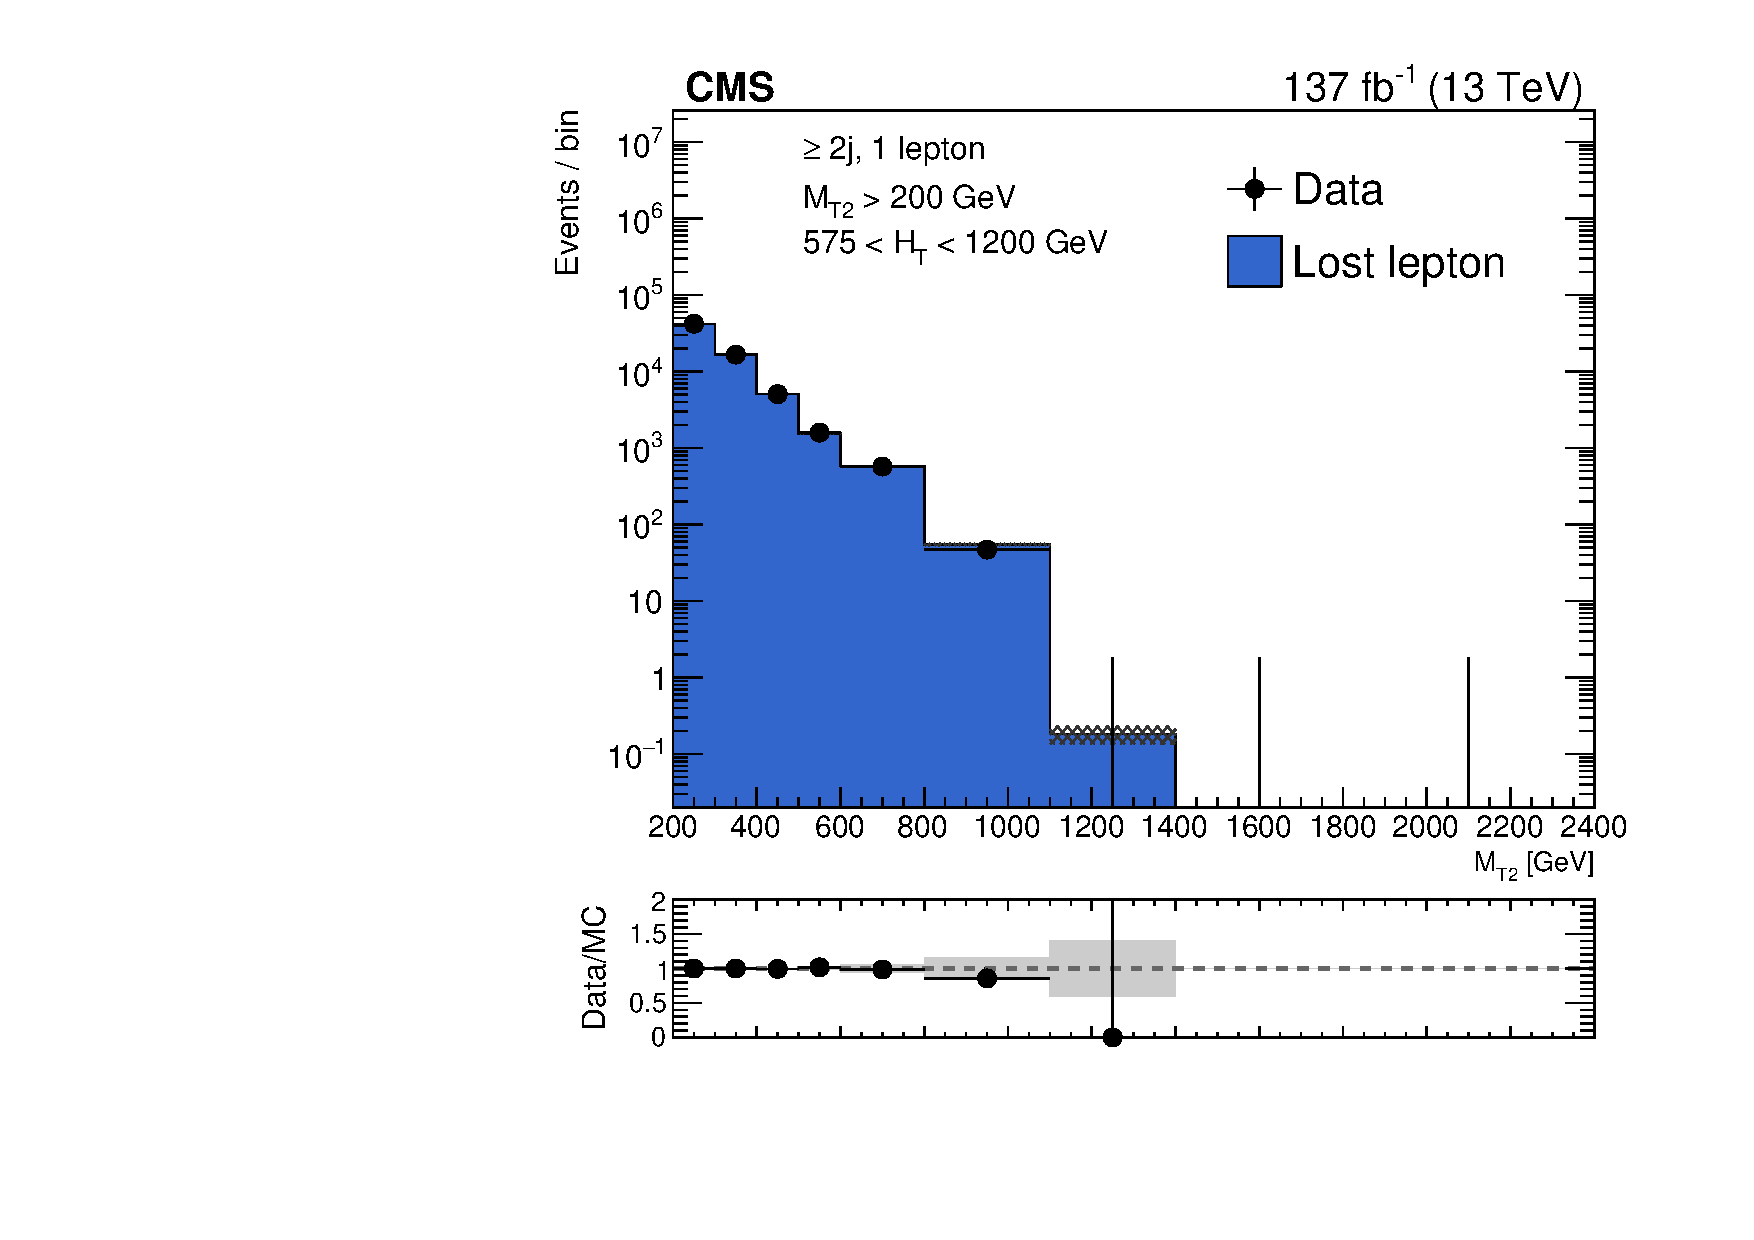
\includegraphics[width=0.47\textwidth]{figs/llep/lostlepHybrid_incl_HT575to1200_mt2bins.pdf}
    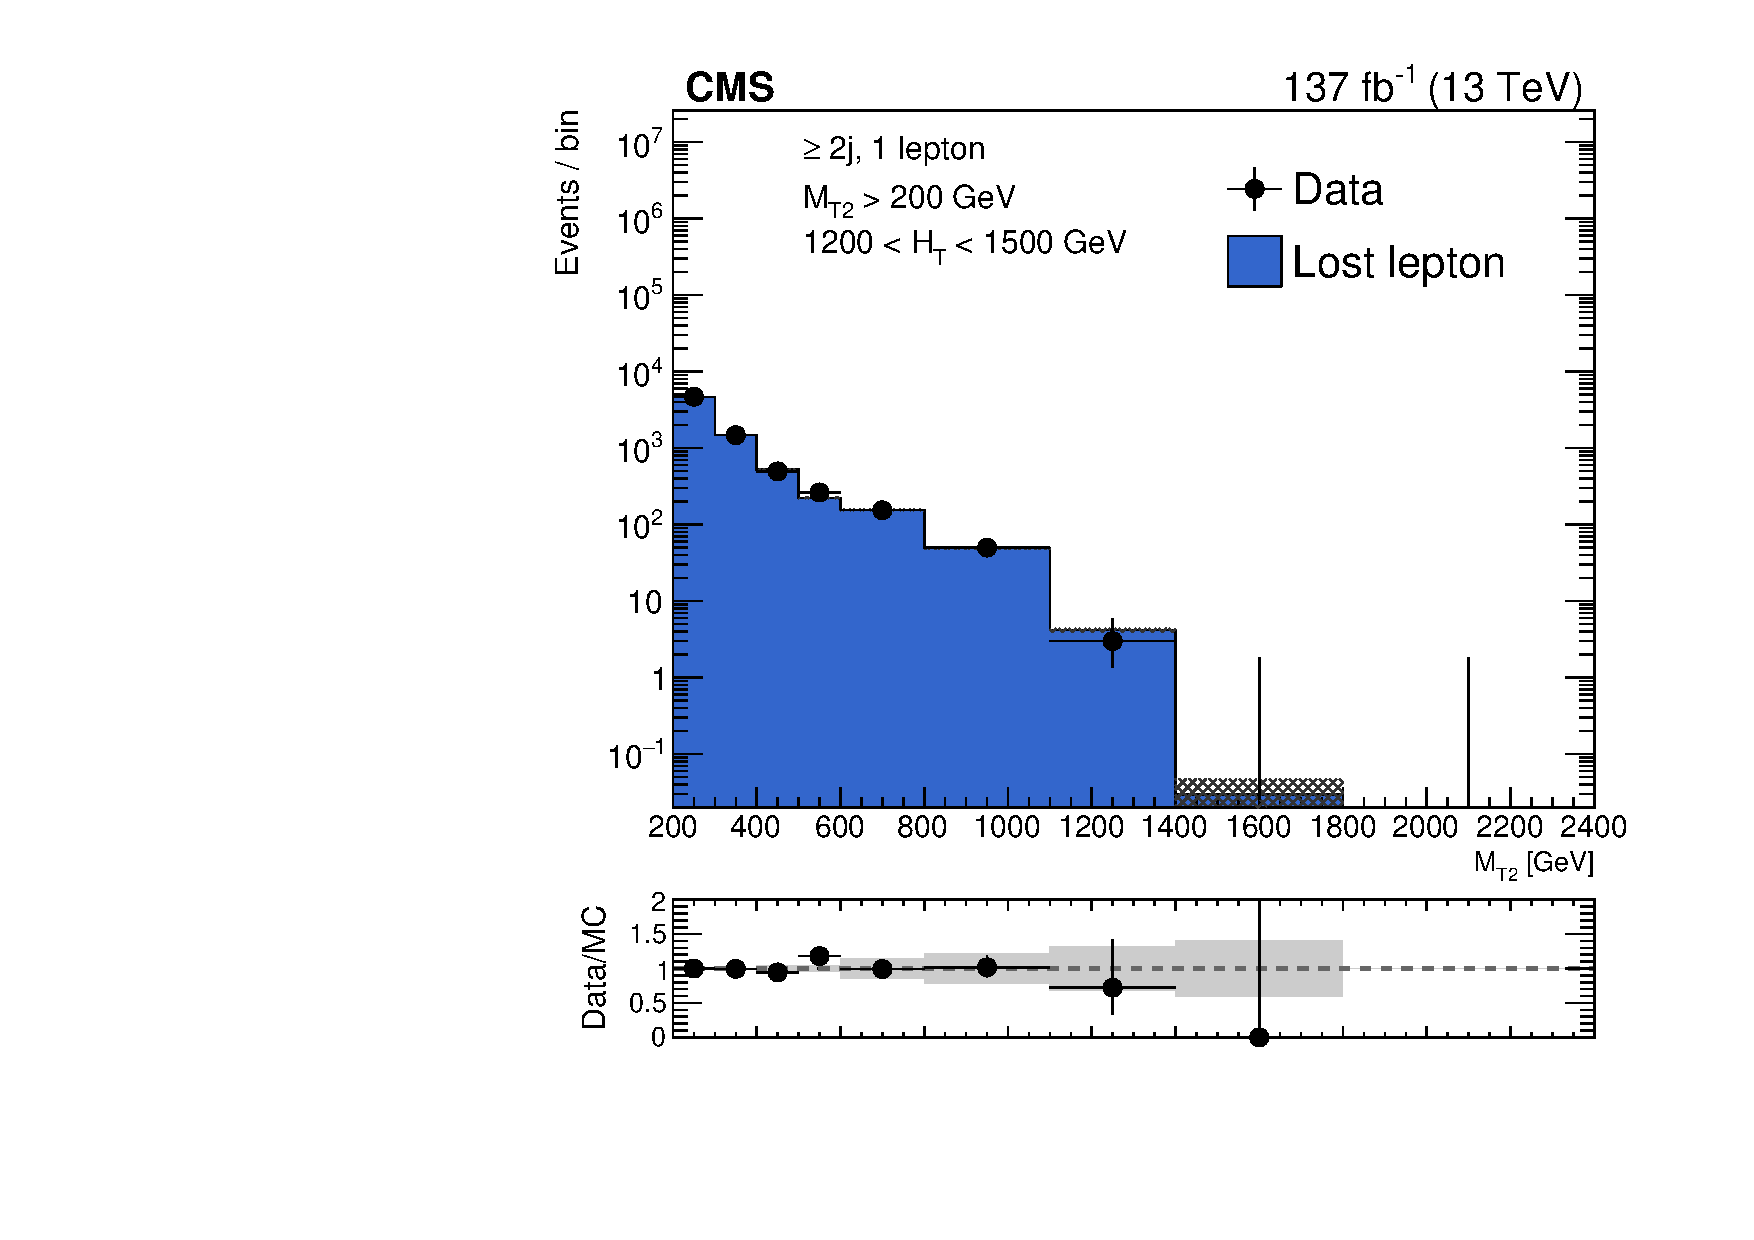
\includegraphics[width=0.47\textwidth]{figs/llep/lostlepHybrid_incl_HT1200to1500_mt2bins.pdf} \\
    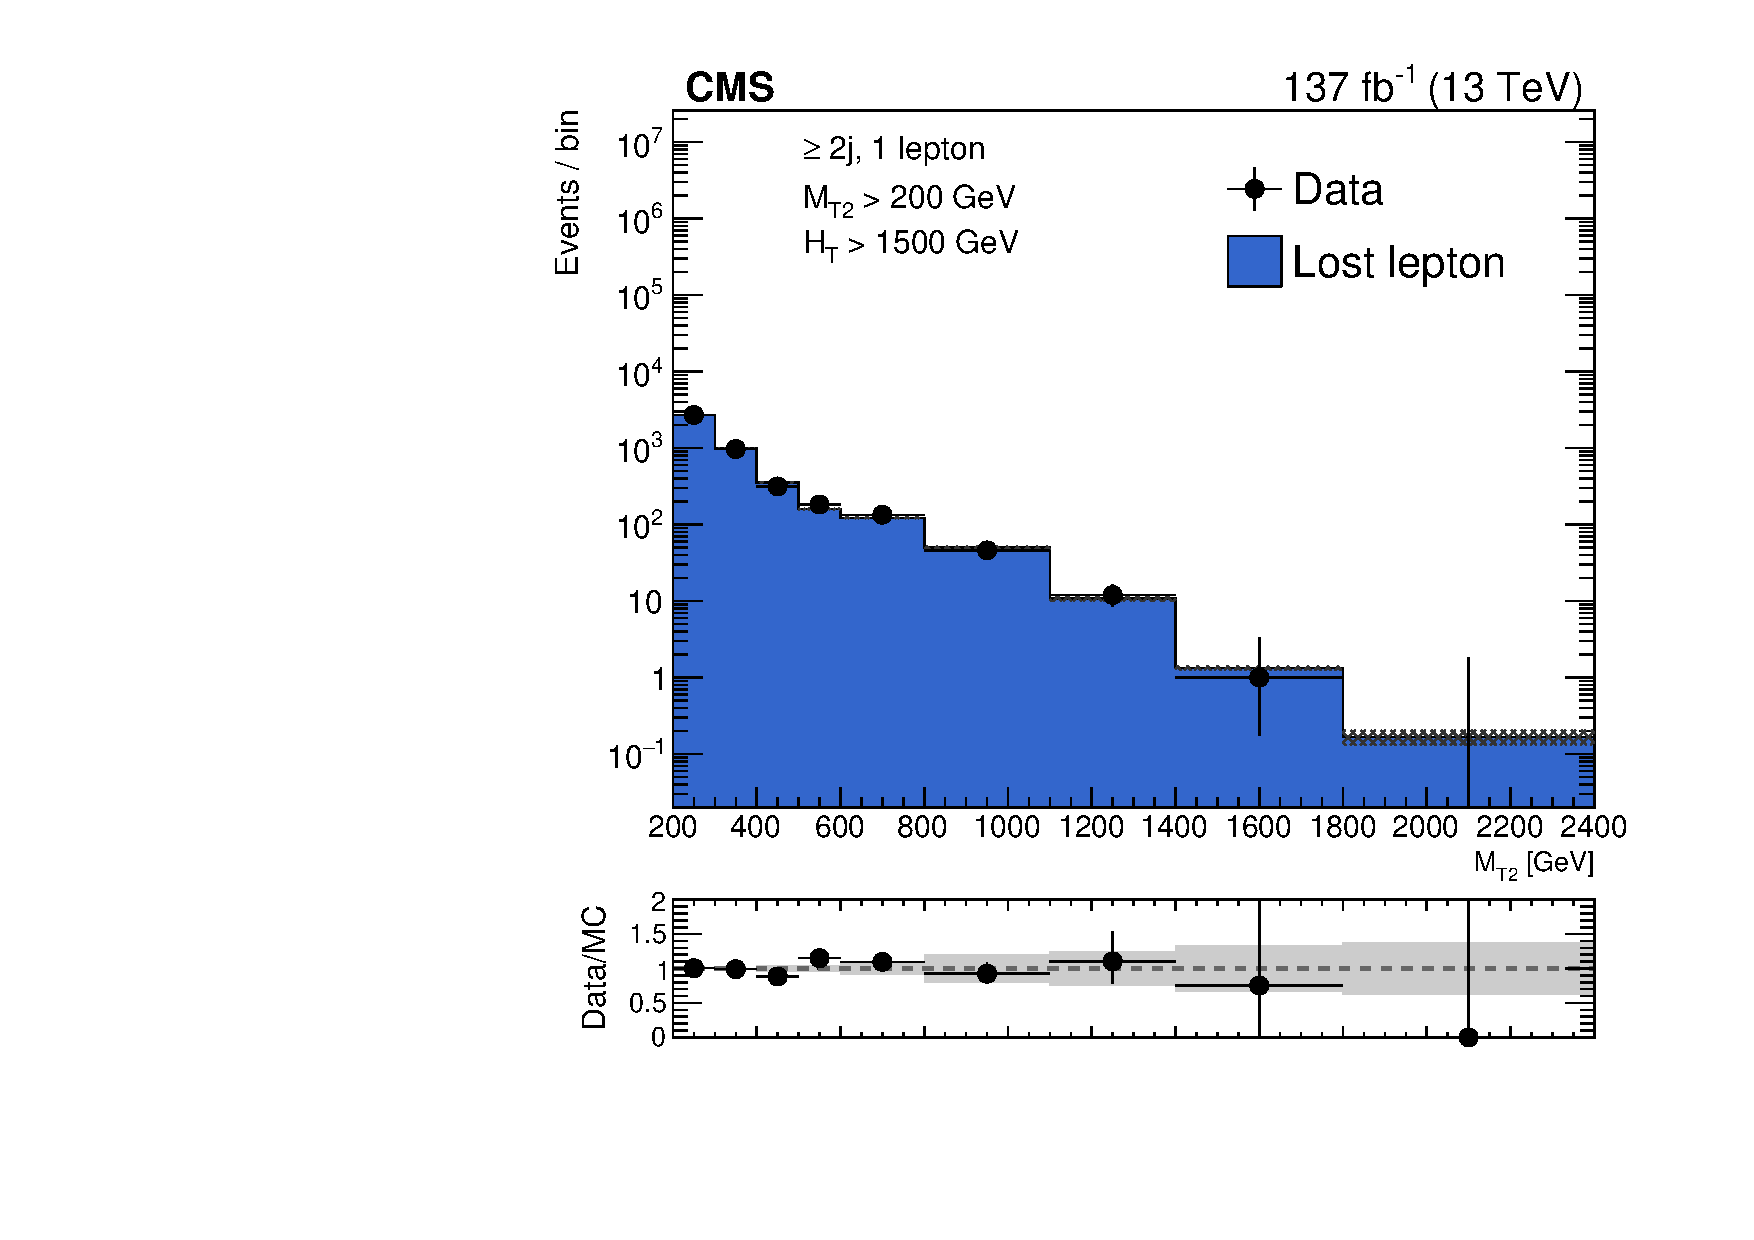
\includegraphics[width=0.47\textwidth]{figs/llep/lostlepHybrid_incl_HTge1500_mt2bins.pdf}
    \caption{The same as Fig.~\ref{fig:llep_mt2dist}, but plotted separately for the Very Low,
      Low, Medium, High, and Extreme \Ht regions.
            }
    \label{fig:llep_mt2dist_ht}
  \end{center}
\end{figure}

% want to include HT-binned plots?

\section{Systematic uncertainties}
\label{sec:llep_syst}

The following systematics are assessed on the lost lepton background prediction:
\begin{itemize}\setlength\itemsep{0mm}
\item Control region statistical error: the Poisson error on the observed data count in each single lepton control region.
This is correlated among all bins that share a common control region (including the \mttwo bins that utilize a merged control region),
but is otherwise uncorrelated.
\item MC statistical error: the statistical uncertainty due to the limited size of the MC samples on the $0\ell/1\ell$ transfer
factor (and on $k_\mrm{LL}(\mttwo)$ for bins in which MC is used to predict the \mttwo shape)
\item $e/\mu$ selection efficiency: to account for differences in lepton efficiency between data and MC, scale factors
are derived in bins of \pt and $\eta$ for electrons and muons by the CMS SUSY group, along with corresponding uncertainties.
These uncertainties are propagated on a per-event basis to the final predicted yield, and the variation is taken as a systematic
uncertainty. This is as large as 7\% and correlated among all bins.
\item $\tau$ selection efficiency: from MC studies, we take a 10\% relative uncertainty on the selection efficiency for 1-prong
$\tau$'s, and a 100\% relative uncertainty on the selection efficiency for 3-prong $\tau$'s. This is propagated to the final predicted
yield and the variation is taken as a systematic uncertainty. This is as large as 3\% and correlated among all bins.
\item $M_\mrm{T}$ cut efficiency: the differences between MC and data of the $M_\mrm{T}$ cut used for the control region
has been studied in a \zll control region in which one lepton is treated as missing (to mimic $W\to\ell\nu$ decay) has been
studied. Based on this, we apply a 3\% systematic uncertainty, correlated everywhere.
\item b tagging efficiency: the CMS b tagging group provides uncertainties on the scale factors used to correct MC b tagging
efficiencies. These are propagated to the final estimate, and the variation is taken as a systematic. This is as large as
4\%, and correlated among all bins.
\item $\ttbar b\bar{b}$ reweighting: as described in Sec.~\ref{sec:llep_ttbb}, MC events with both \ttbar and $b\bar{b}$ pairs
are weighted by an additional factor of $1.7\pm0.5$. This uncertainty is propagated to the final estimate, and the variation is
taken as a systematic uncertainty. The magnitude of this uncertainty is from 0--25\% (largest in bins with very high \Nj and \Nb),
and correlated everywhere.
\item jet energy scale: from MC studies using the jet energy correction uncertainties provided by the CMS JetMET group, 
we apply a 5\% uncertainty, correlated among all bins.
\item MC renormalization/factorization scales: derived by varying the generator weight of the MC. This is typically a few percent but
up to 10\% in some bins, and correlated everywhere.
\item \mttwo shape uncertainty: much like for the \znunu estimate, this is an extra uncertainty assigned to the \mttwo shape,
accounting for both theoretical and experimental effects. It is based on MC variation studies and validated using the \mttwo
shape comparisons shown in Figs.~\ref{fig:llep_mt2dist} and \ref{fig:llep_mt2dist_ht} (solid gray band in ratio plot). The
uncertainty is implemented as a linear morphing of the \mttwo shape, starting from the first \mttwo bin in each topological region
where the MC shape is used, and growing to a maximum of 40\% in the last \mttwo bin. This uncertainty is correlated within
a given topological region, but not between different topological regions.

\end{itemize}
